\documentclass[../presentation.tex]{subfiles} % Parent file
\graphicspath{{\subfix{../images/}}} % Images path

\begin{document}

\section{Segmentation}

\begin{frame}
	\begin{cbox}
		{\fontsize{20pt}{7.2}\selectfont Segmentation}
	\end{cbox}
\end{frame}


% Slide 1 ──────────────────────────────────────────────────────────────────────
\begin{frame}[t]

	\frametitle{U-Net Models}

	$3$ models for the segmentation task:

	\begin{itemize}
		\setlength{\itemsep}{0.8ex}
		\only<1->{\item \bft{Classic U-Net}: \itt{\gray{baseline U-Net model
		architecture}}}
		\only<2->{\item \bft{Improved U-Net}: \itt{\gray{small improvements, fewer
		parameters}}}
		\only<3->{\item \bft{Attention U-Net}: \itt{\gray{attention mechanism
		added}}}
\end{itemize}

	\vspace{-2ex}

	\only<4->{
		\begin{figure}
			\centering
			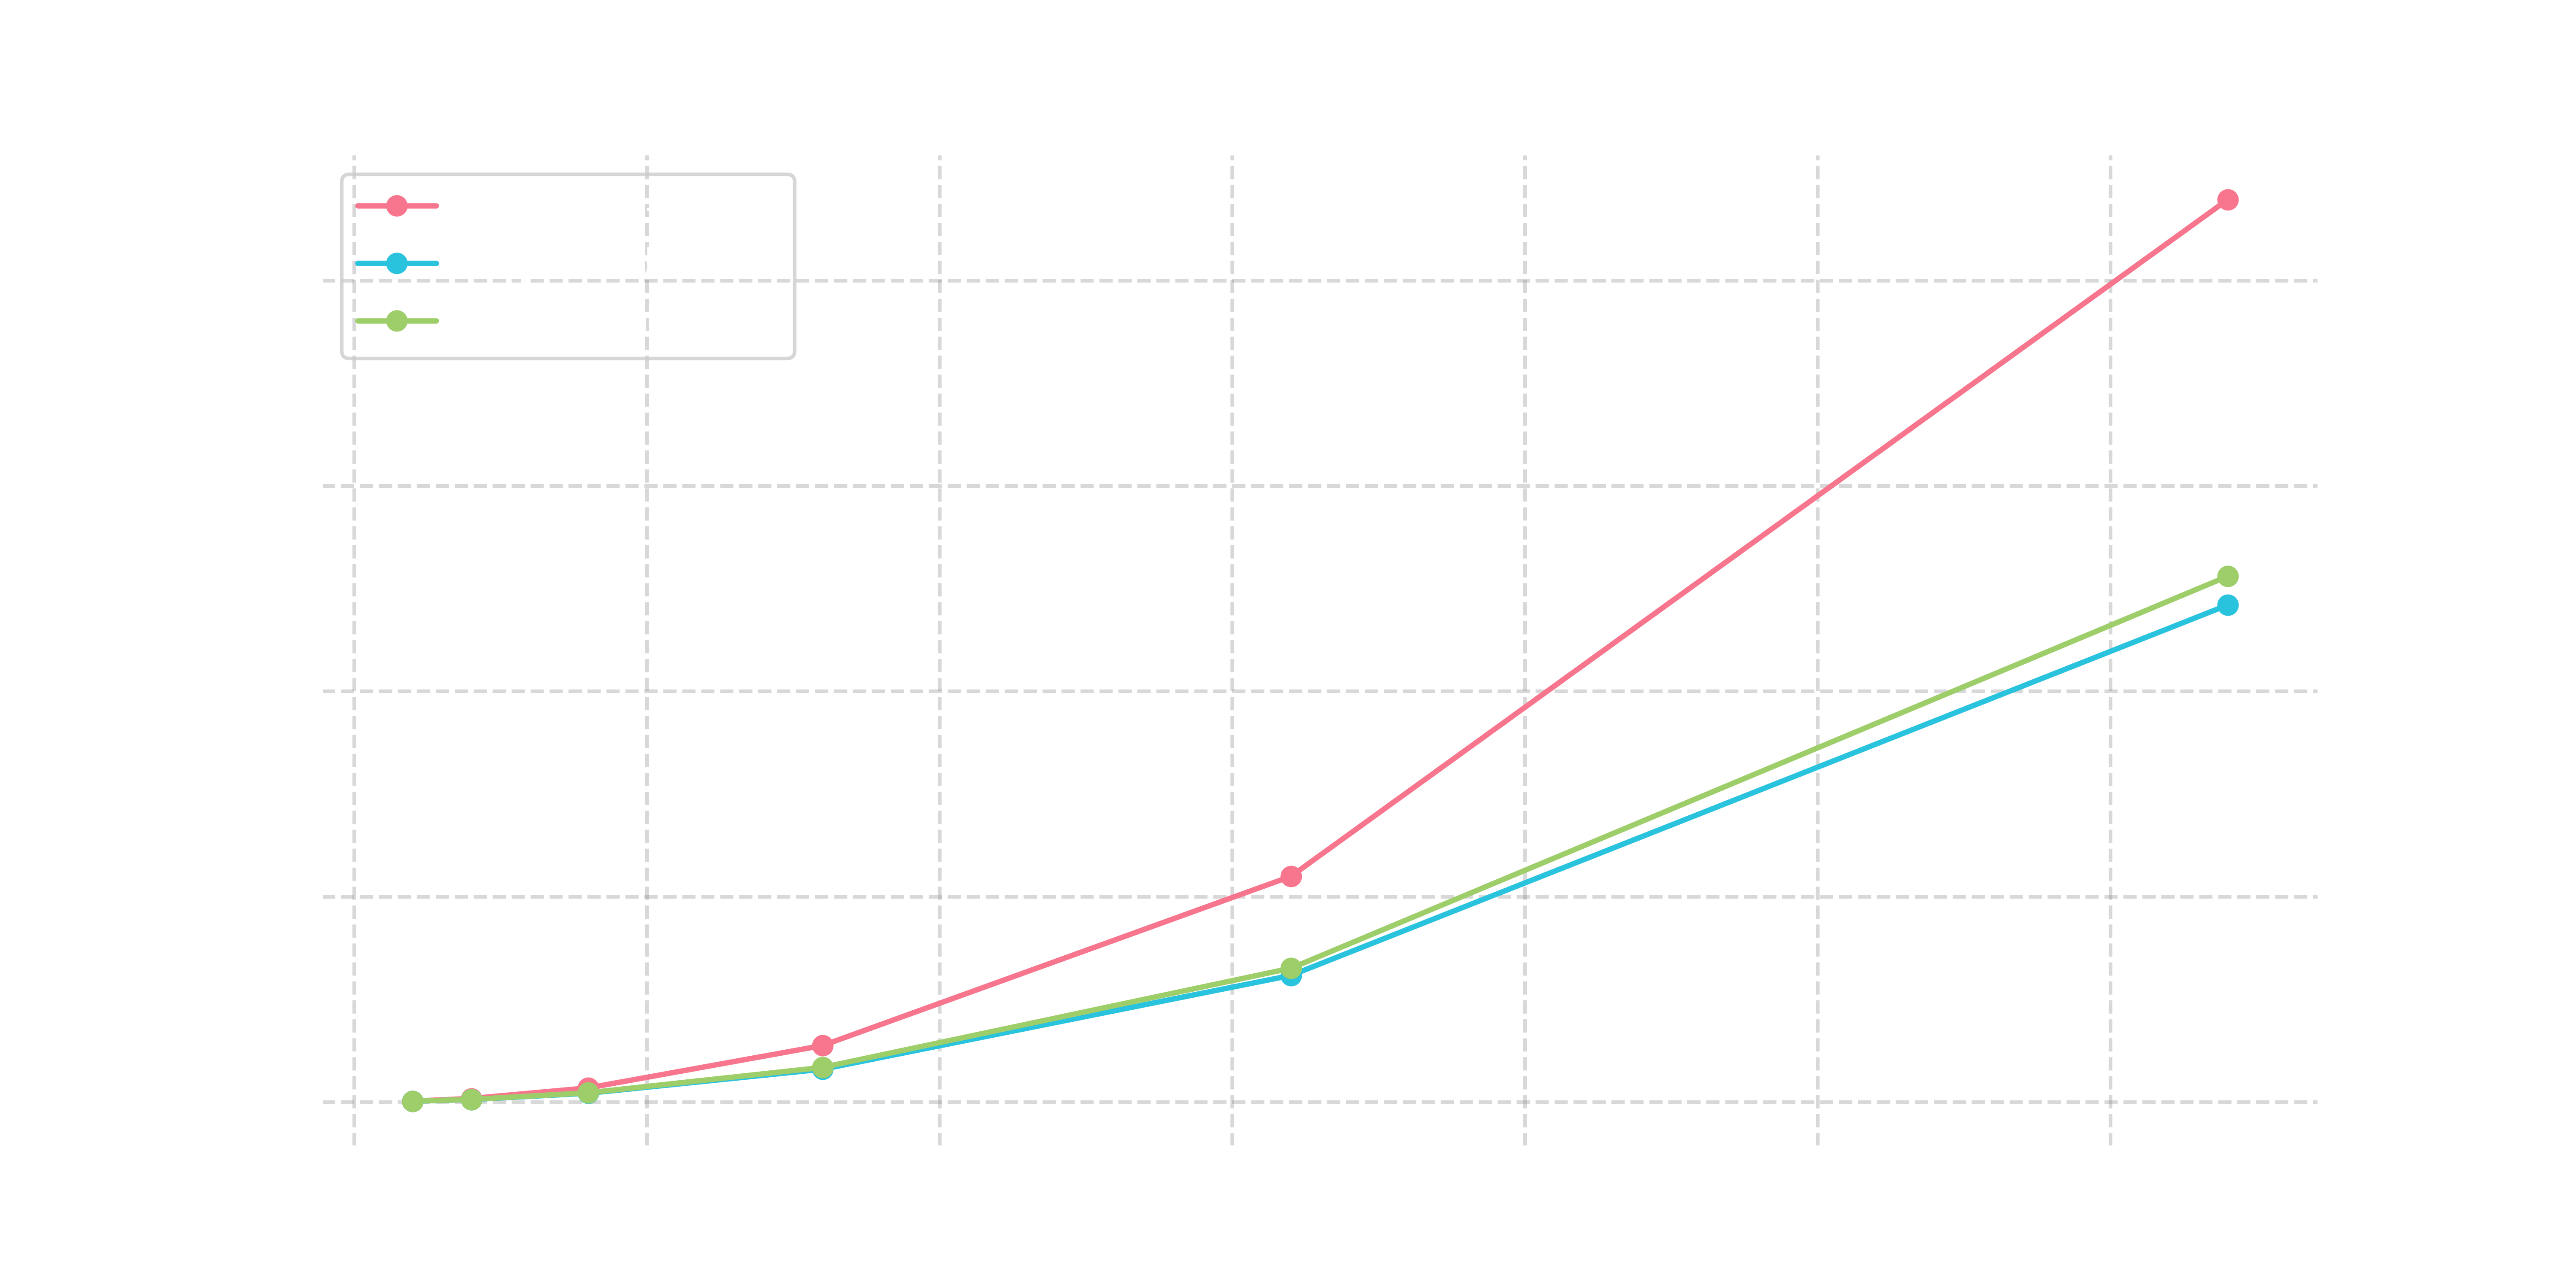
\includegraphics[width=\textwidth]{parameters_vs_filters.png}
		\end{figure}
	}

\end{frame}


% Slide 2 ──────────────────────────────────────────────────────────────────────
\begin{frame}

	\frametitle{Classic U-Net}

	\centering

	\begin{tikzpicture}[remember picture,overlay]
			% Adjust the position of the image
			\node[anchor=south] at ($(current page.south) + (0, 0.4)$) {
				\only<1>{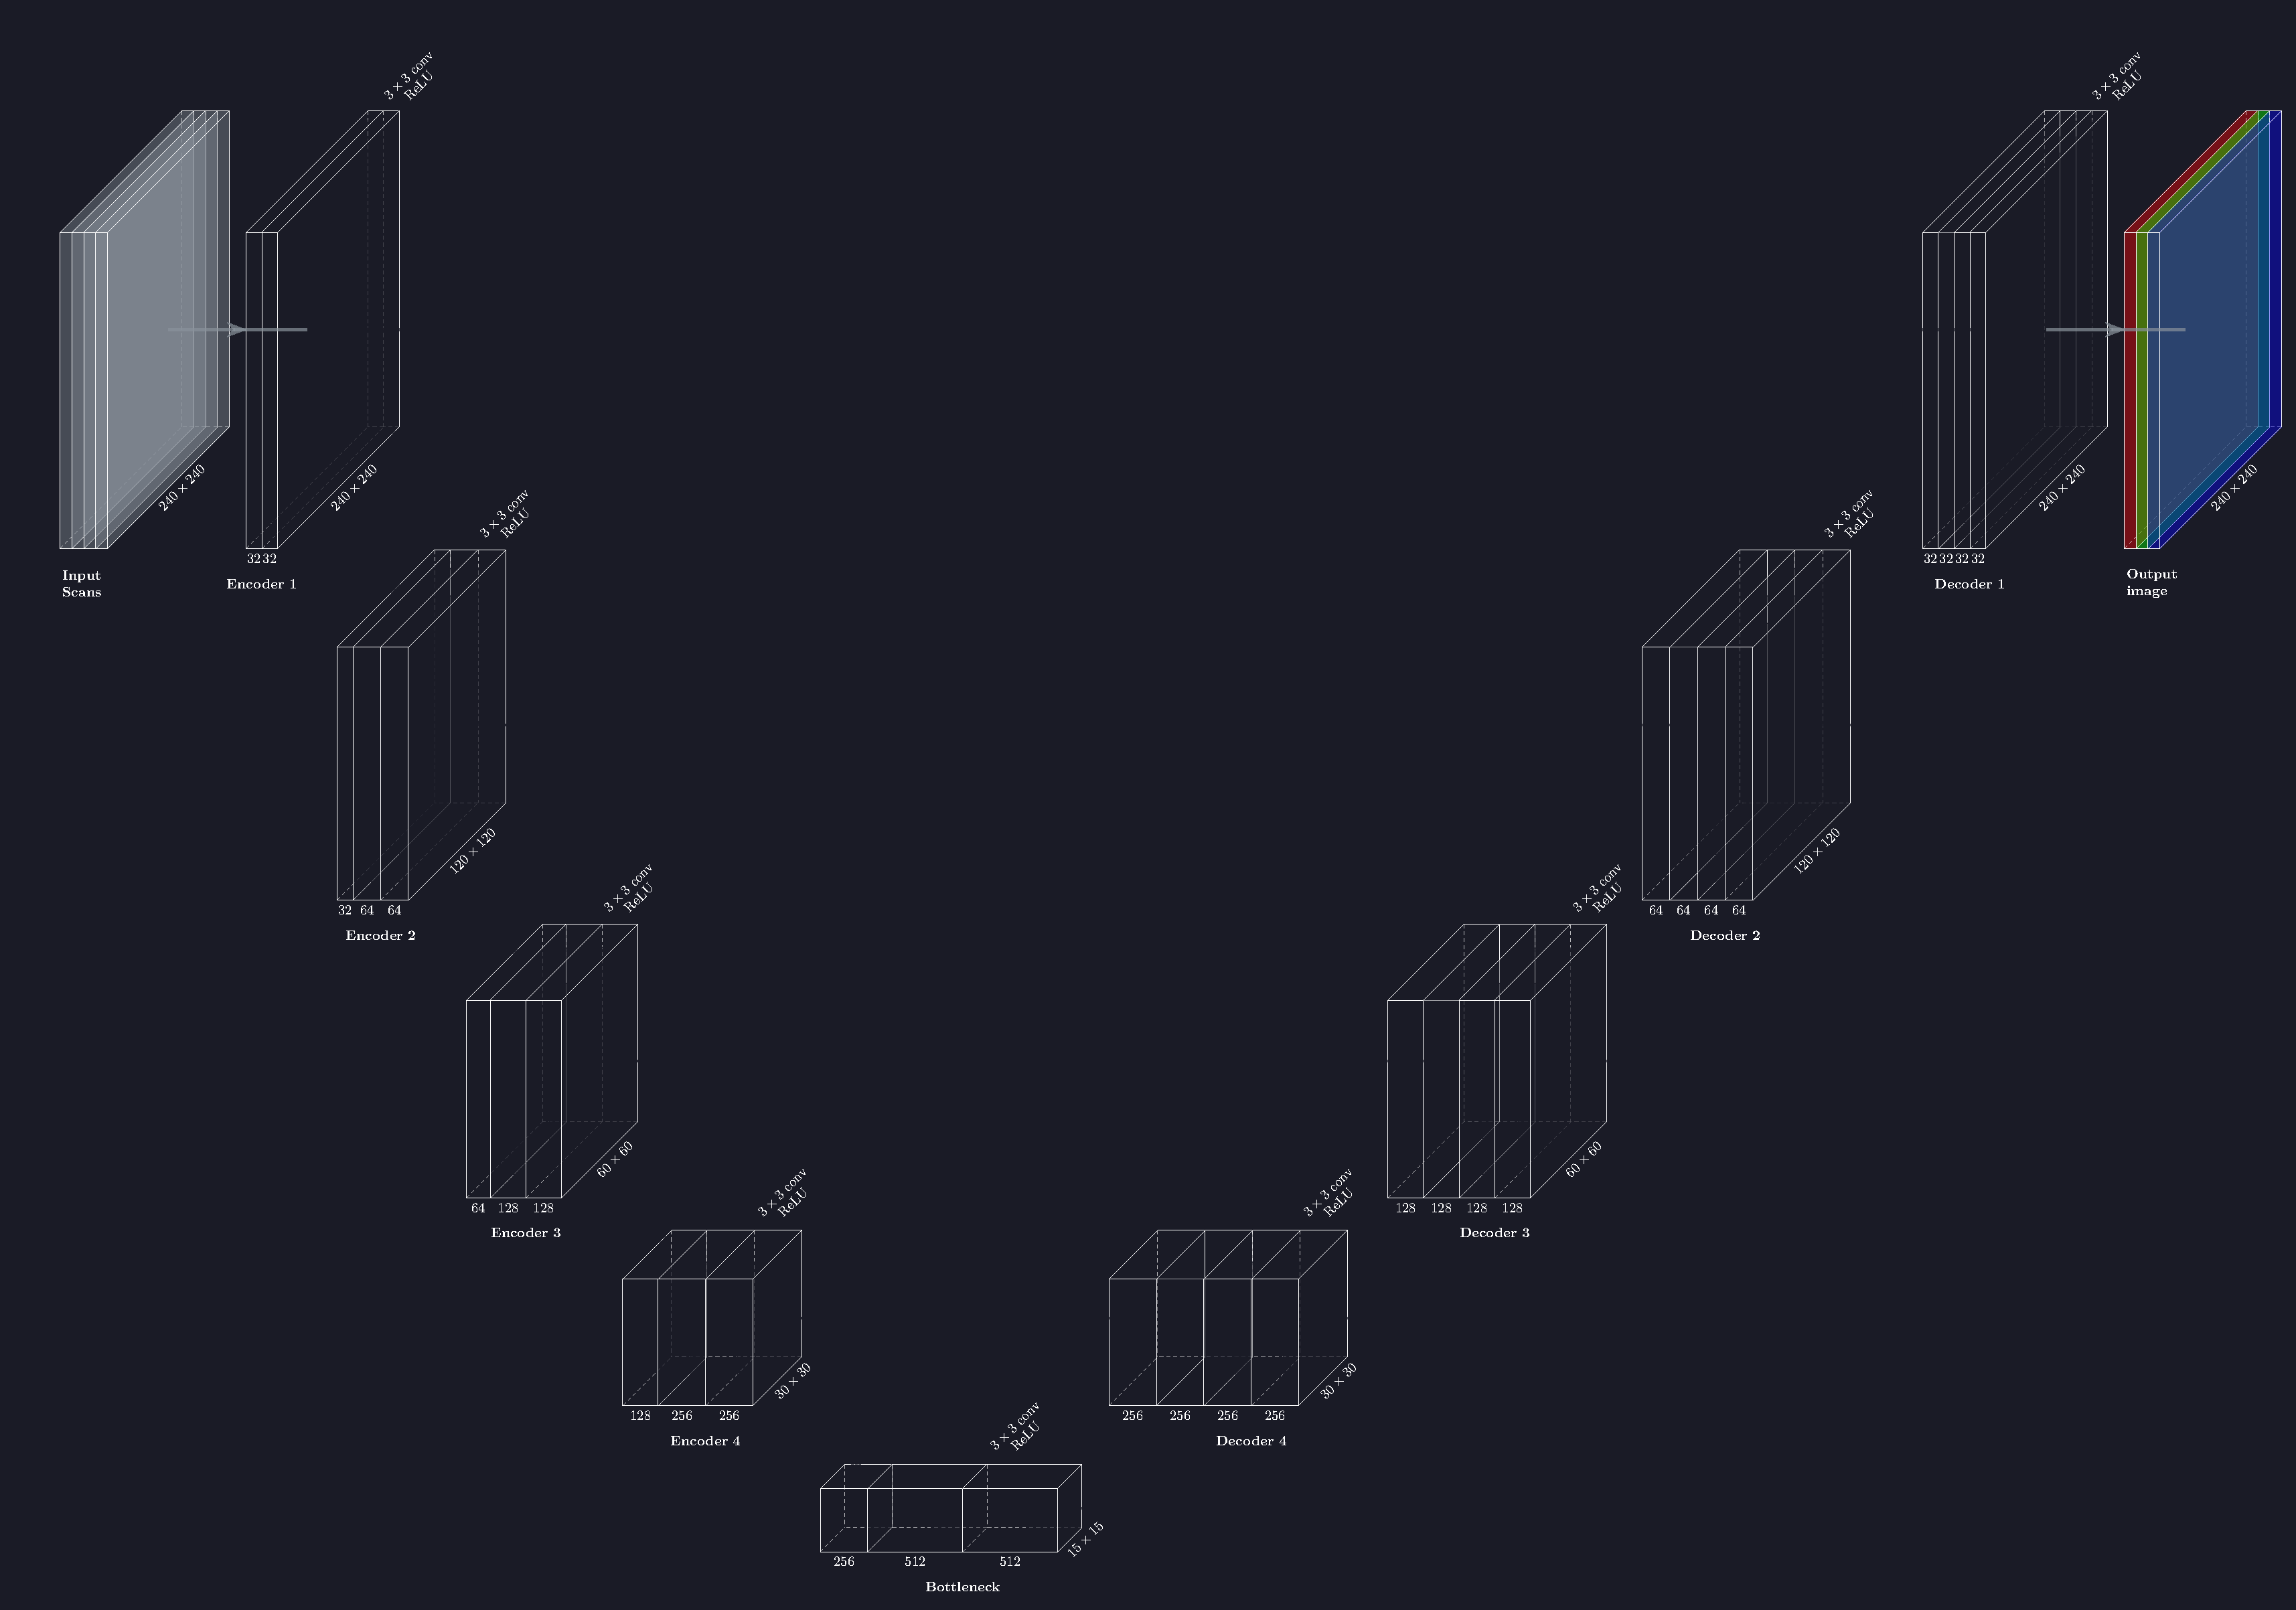
\includegraphics[width=\textwidth]{classic-unet-1.pdf}}%
				\only<2>{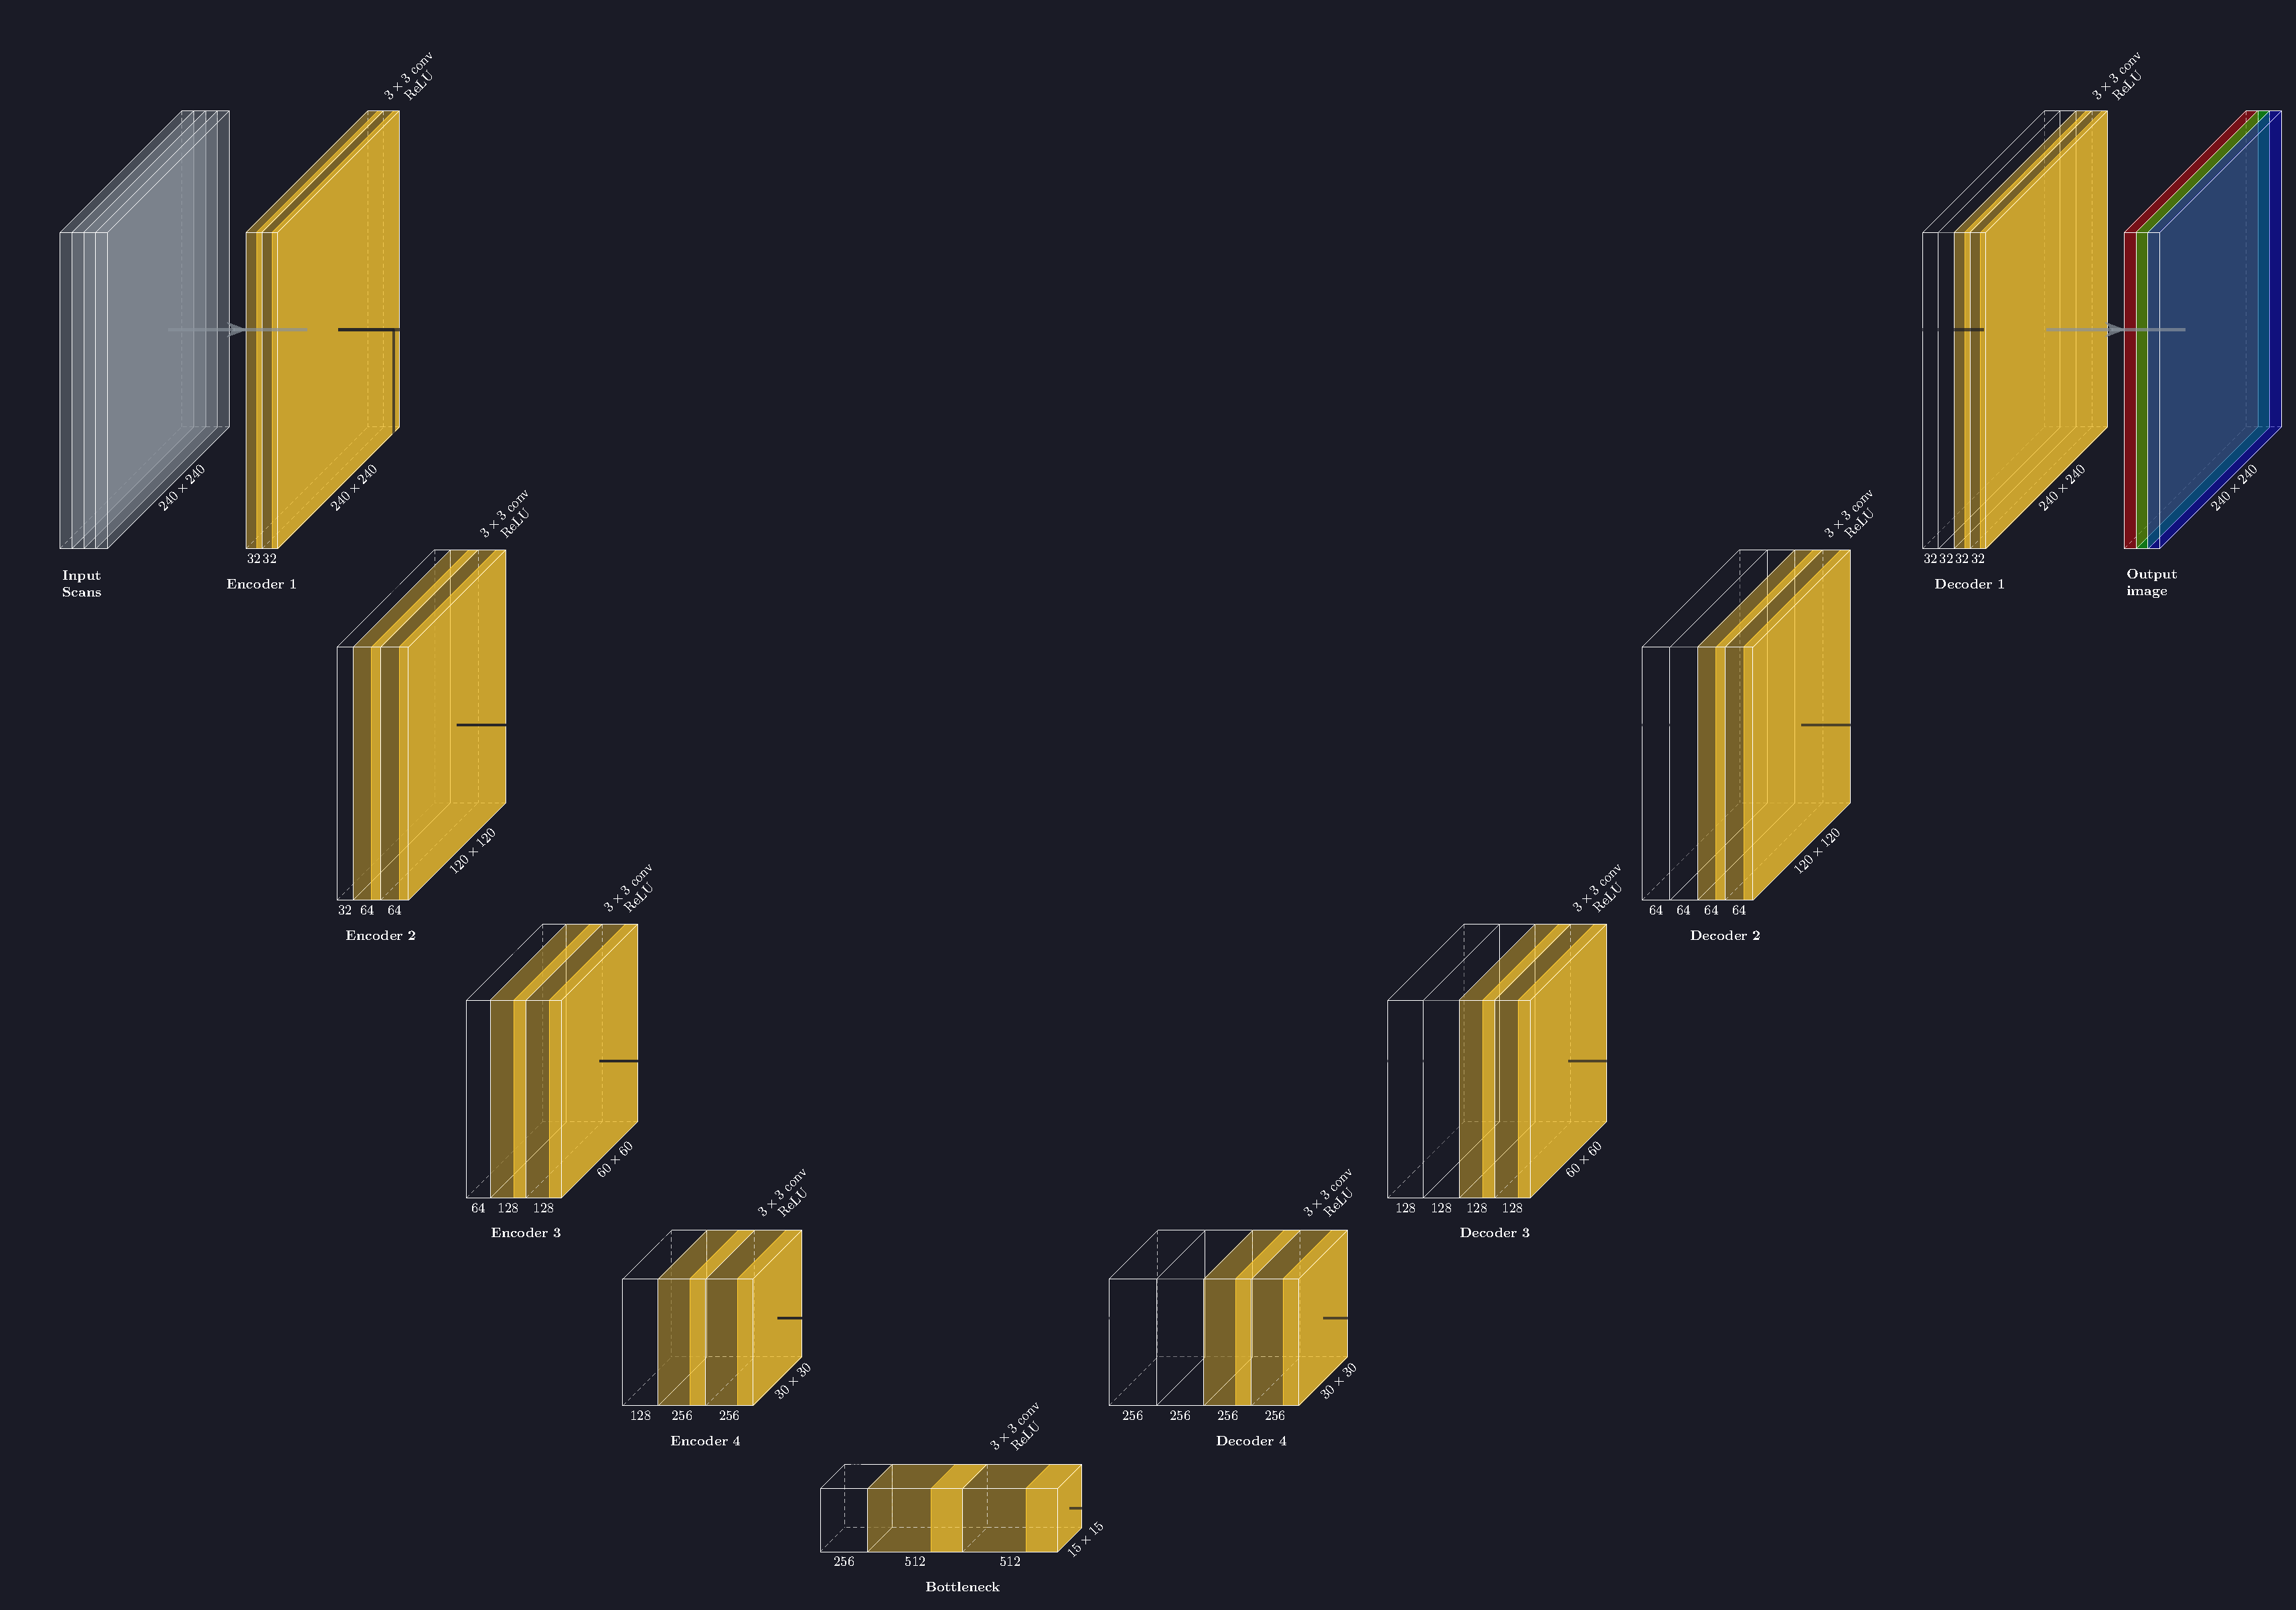
\includegraphics[width=\textwidth]{classic-unet-2.pdf}}%
				\only<3>{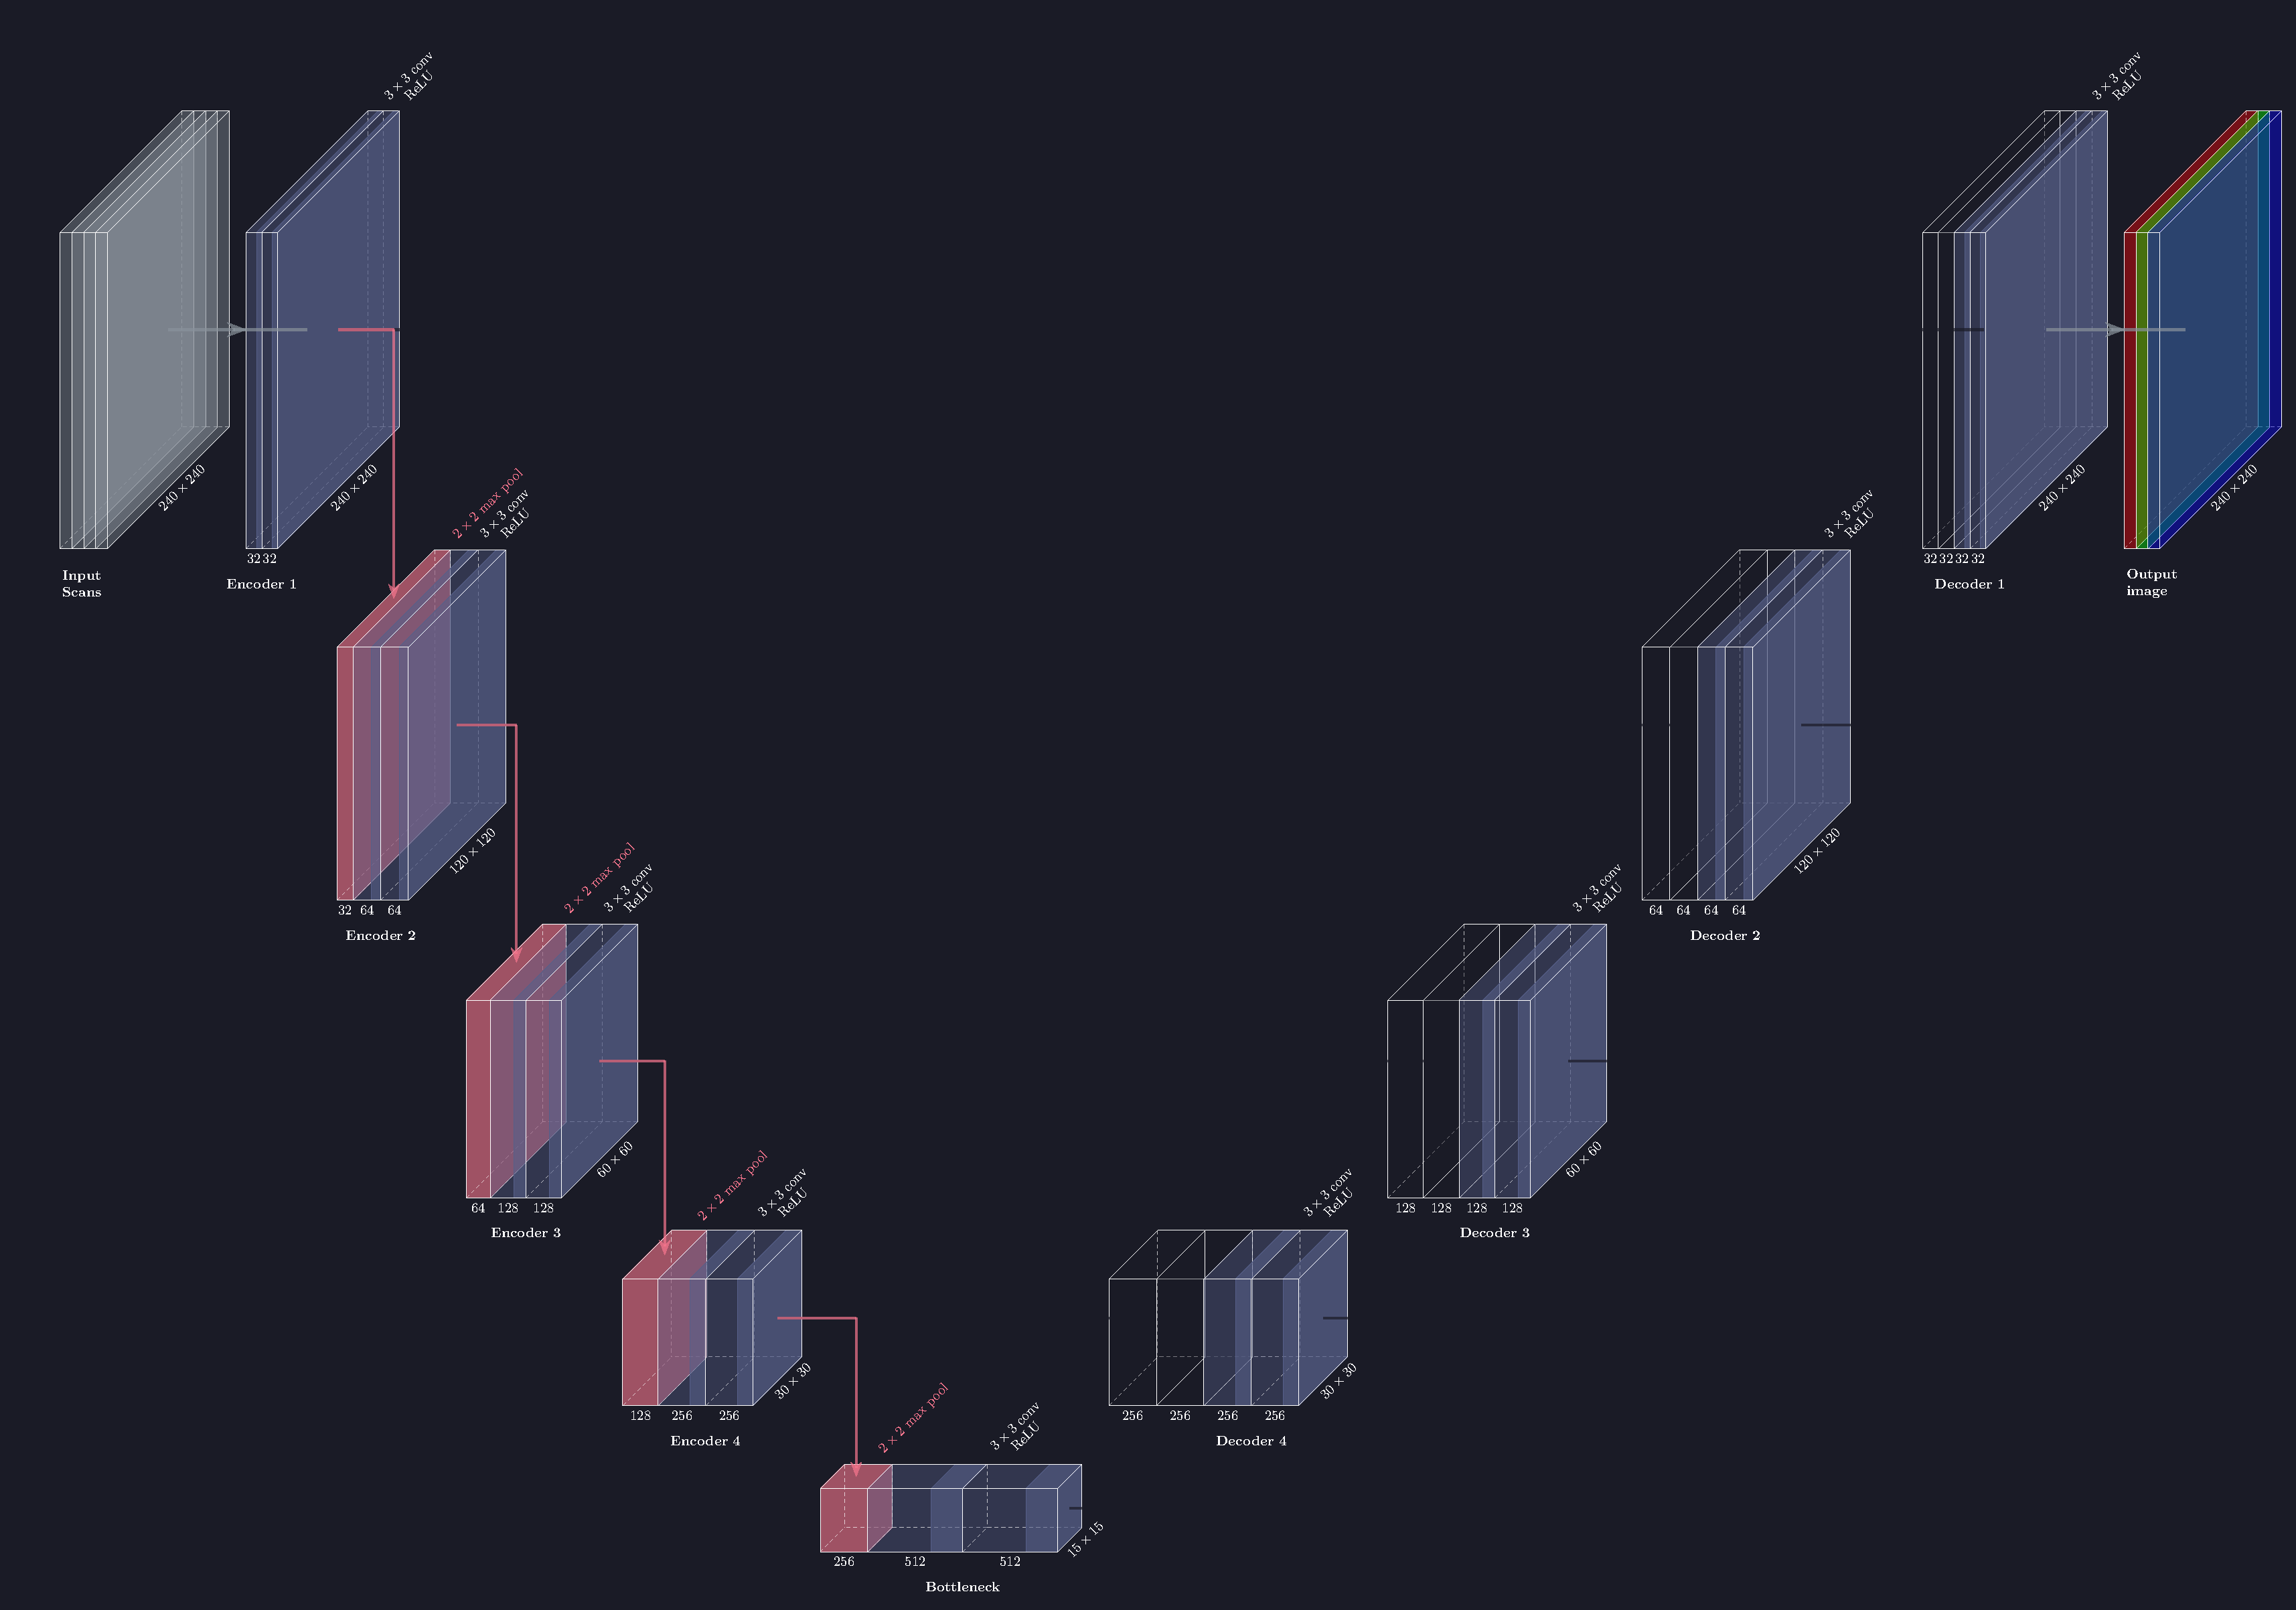
\includegraphics[width=\textwidth]{classic-unet-3.pdf}}%
				\only<4>{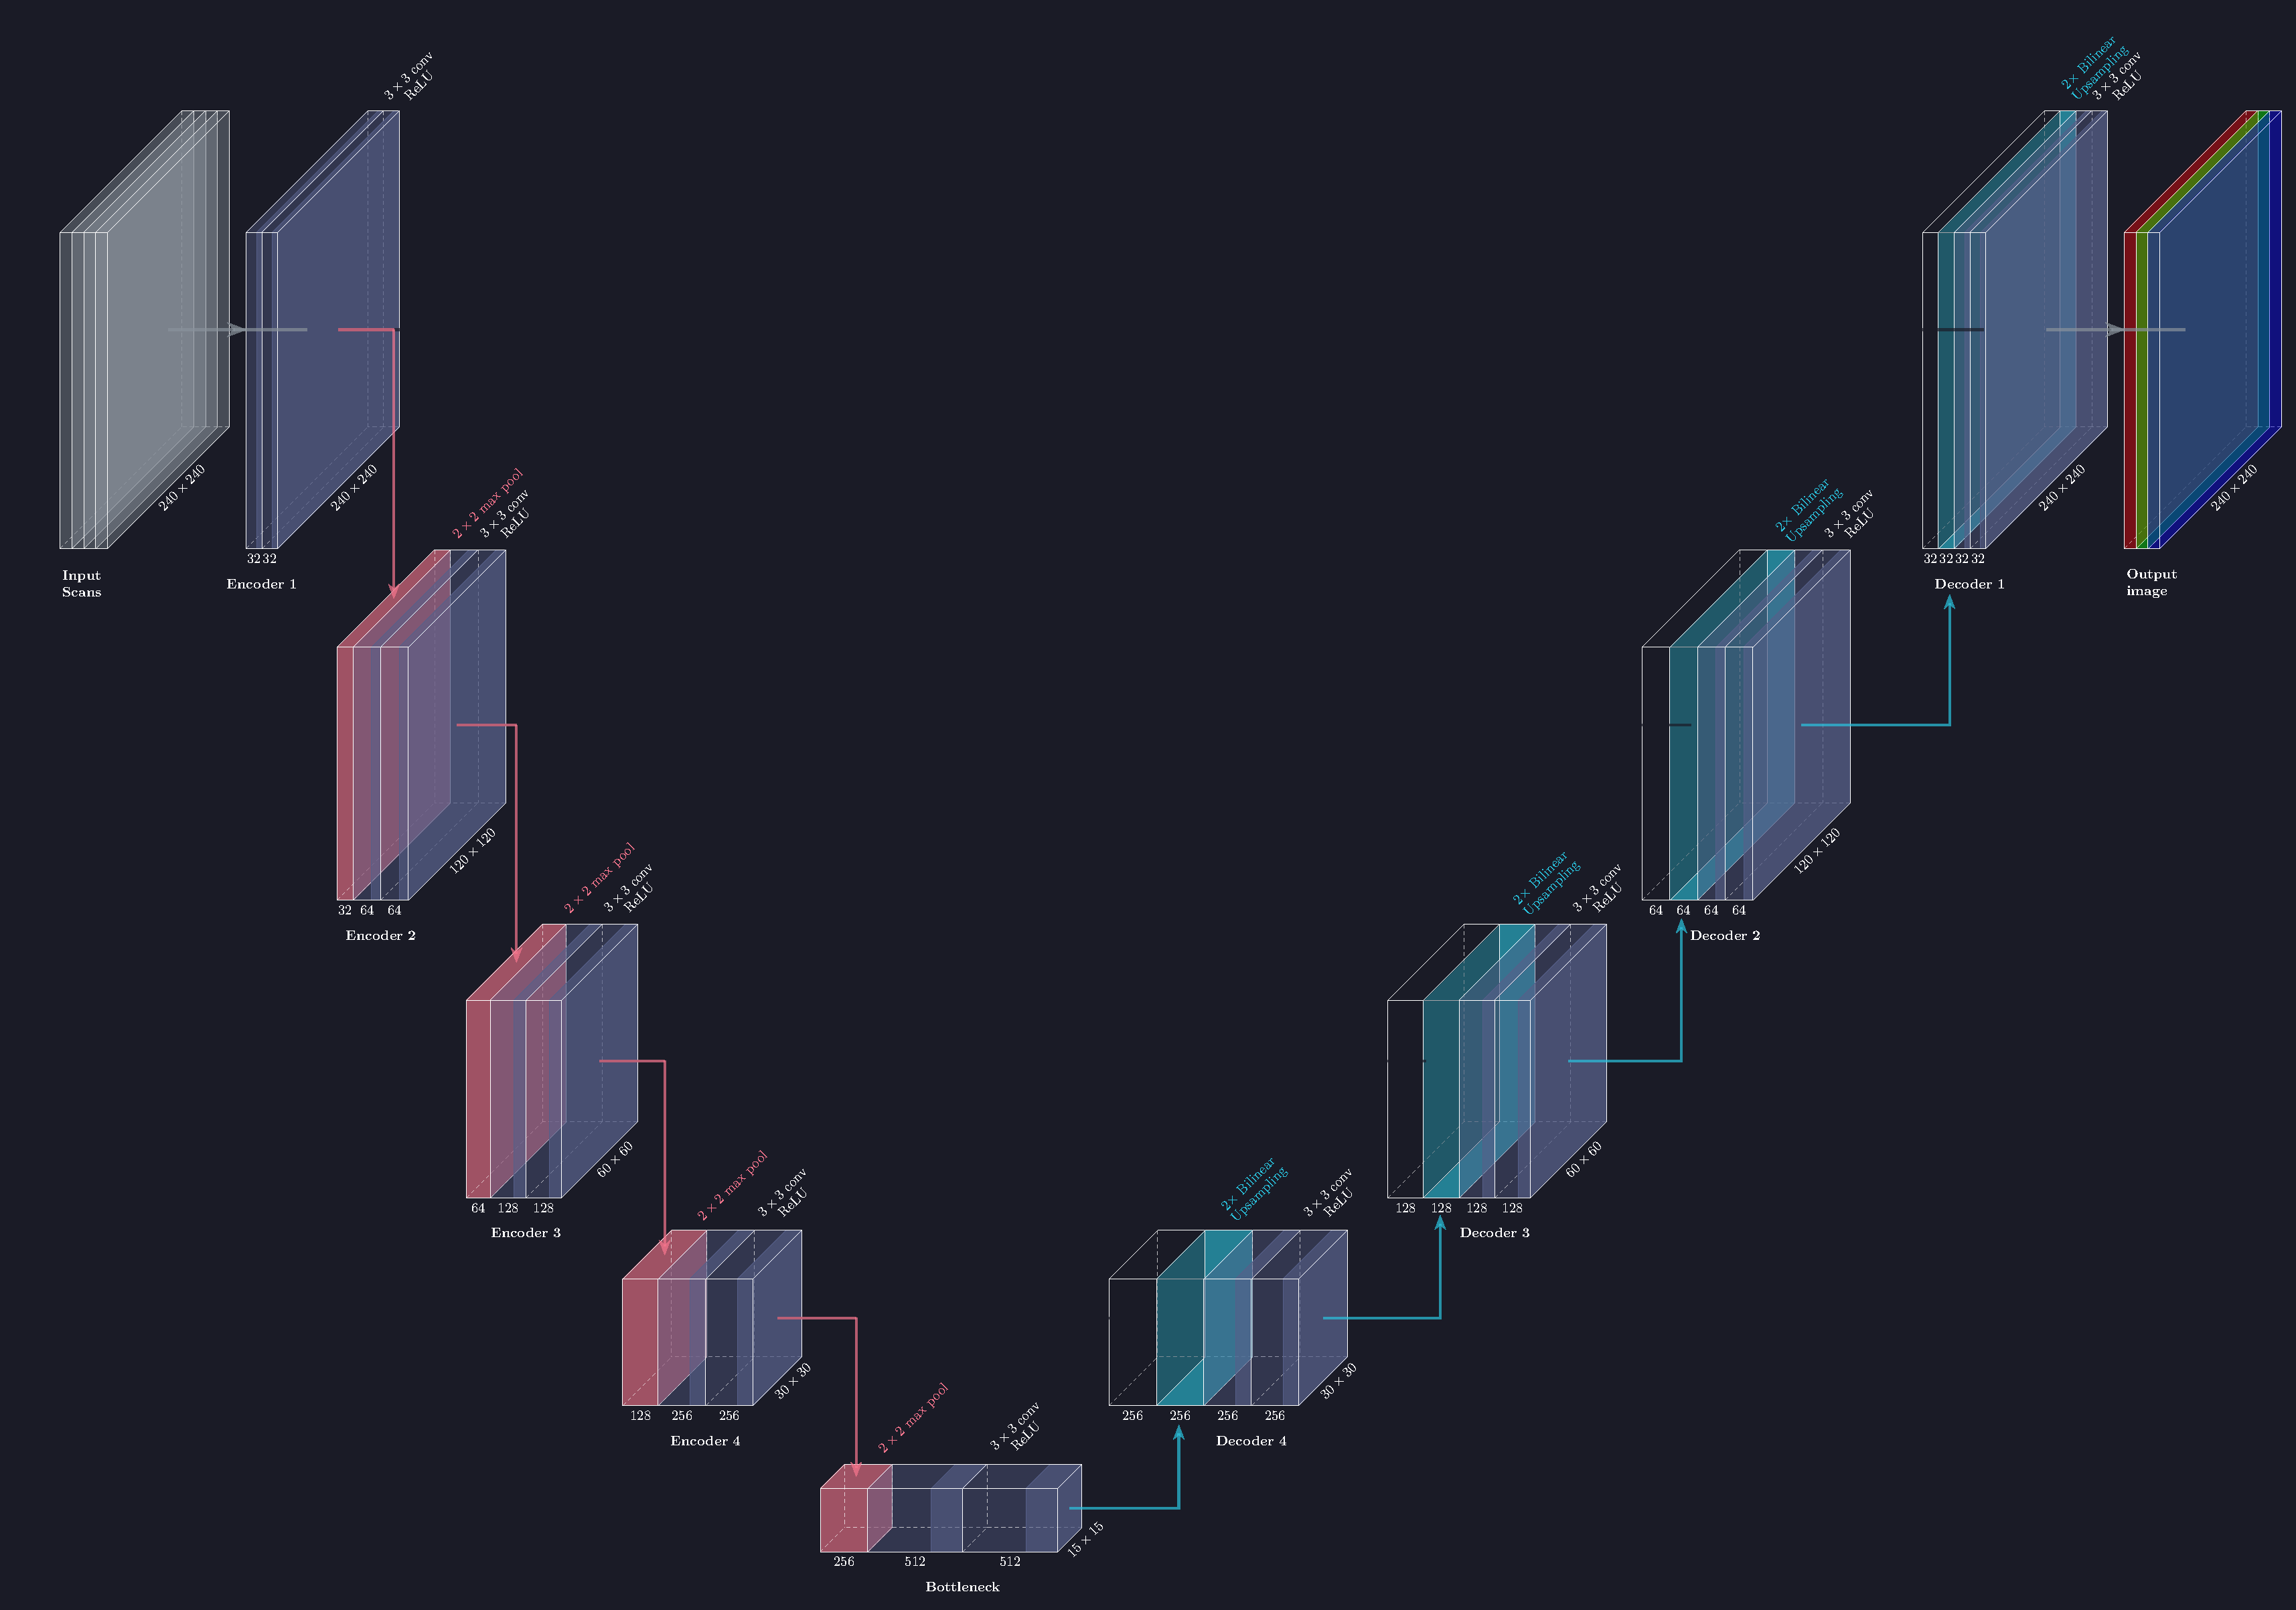
\includegraphics[width=\textwidth]{classic-unet-4.pdf}}%
				\only<5>{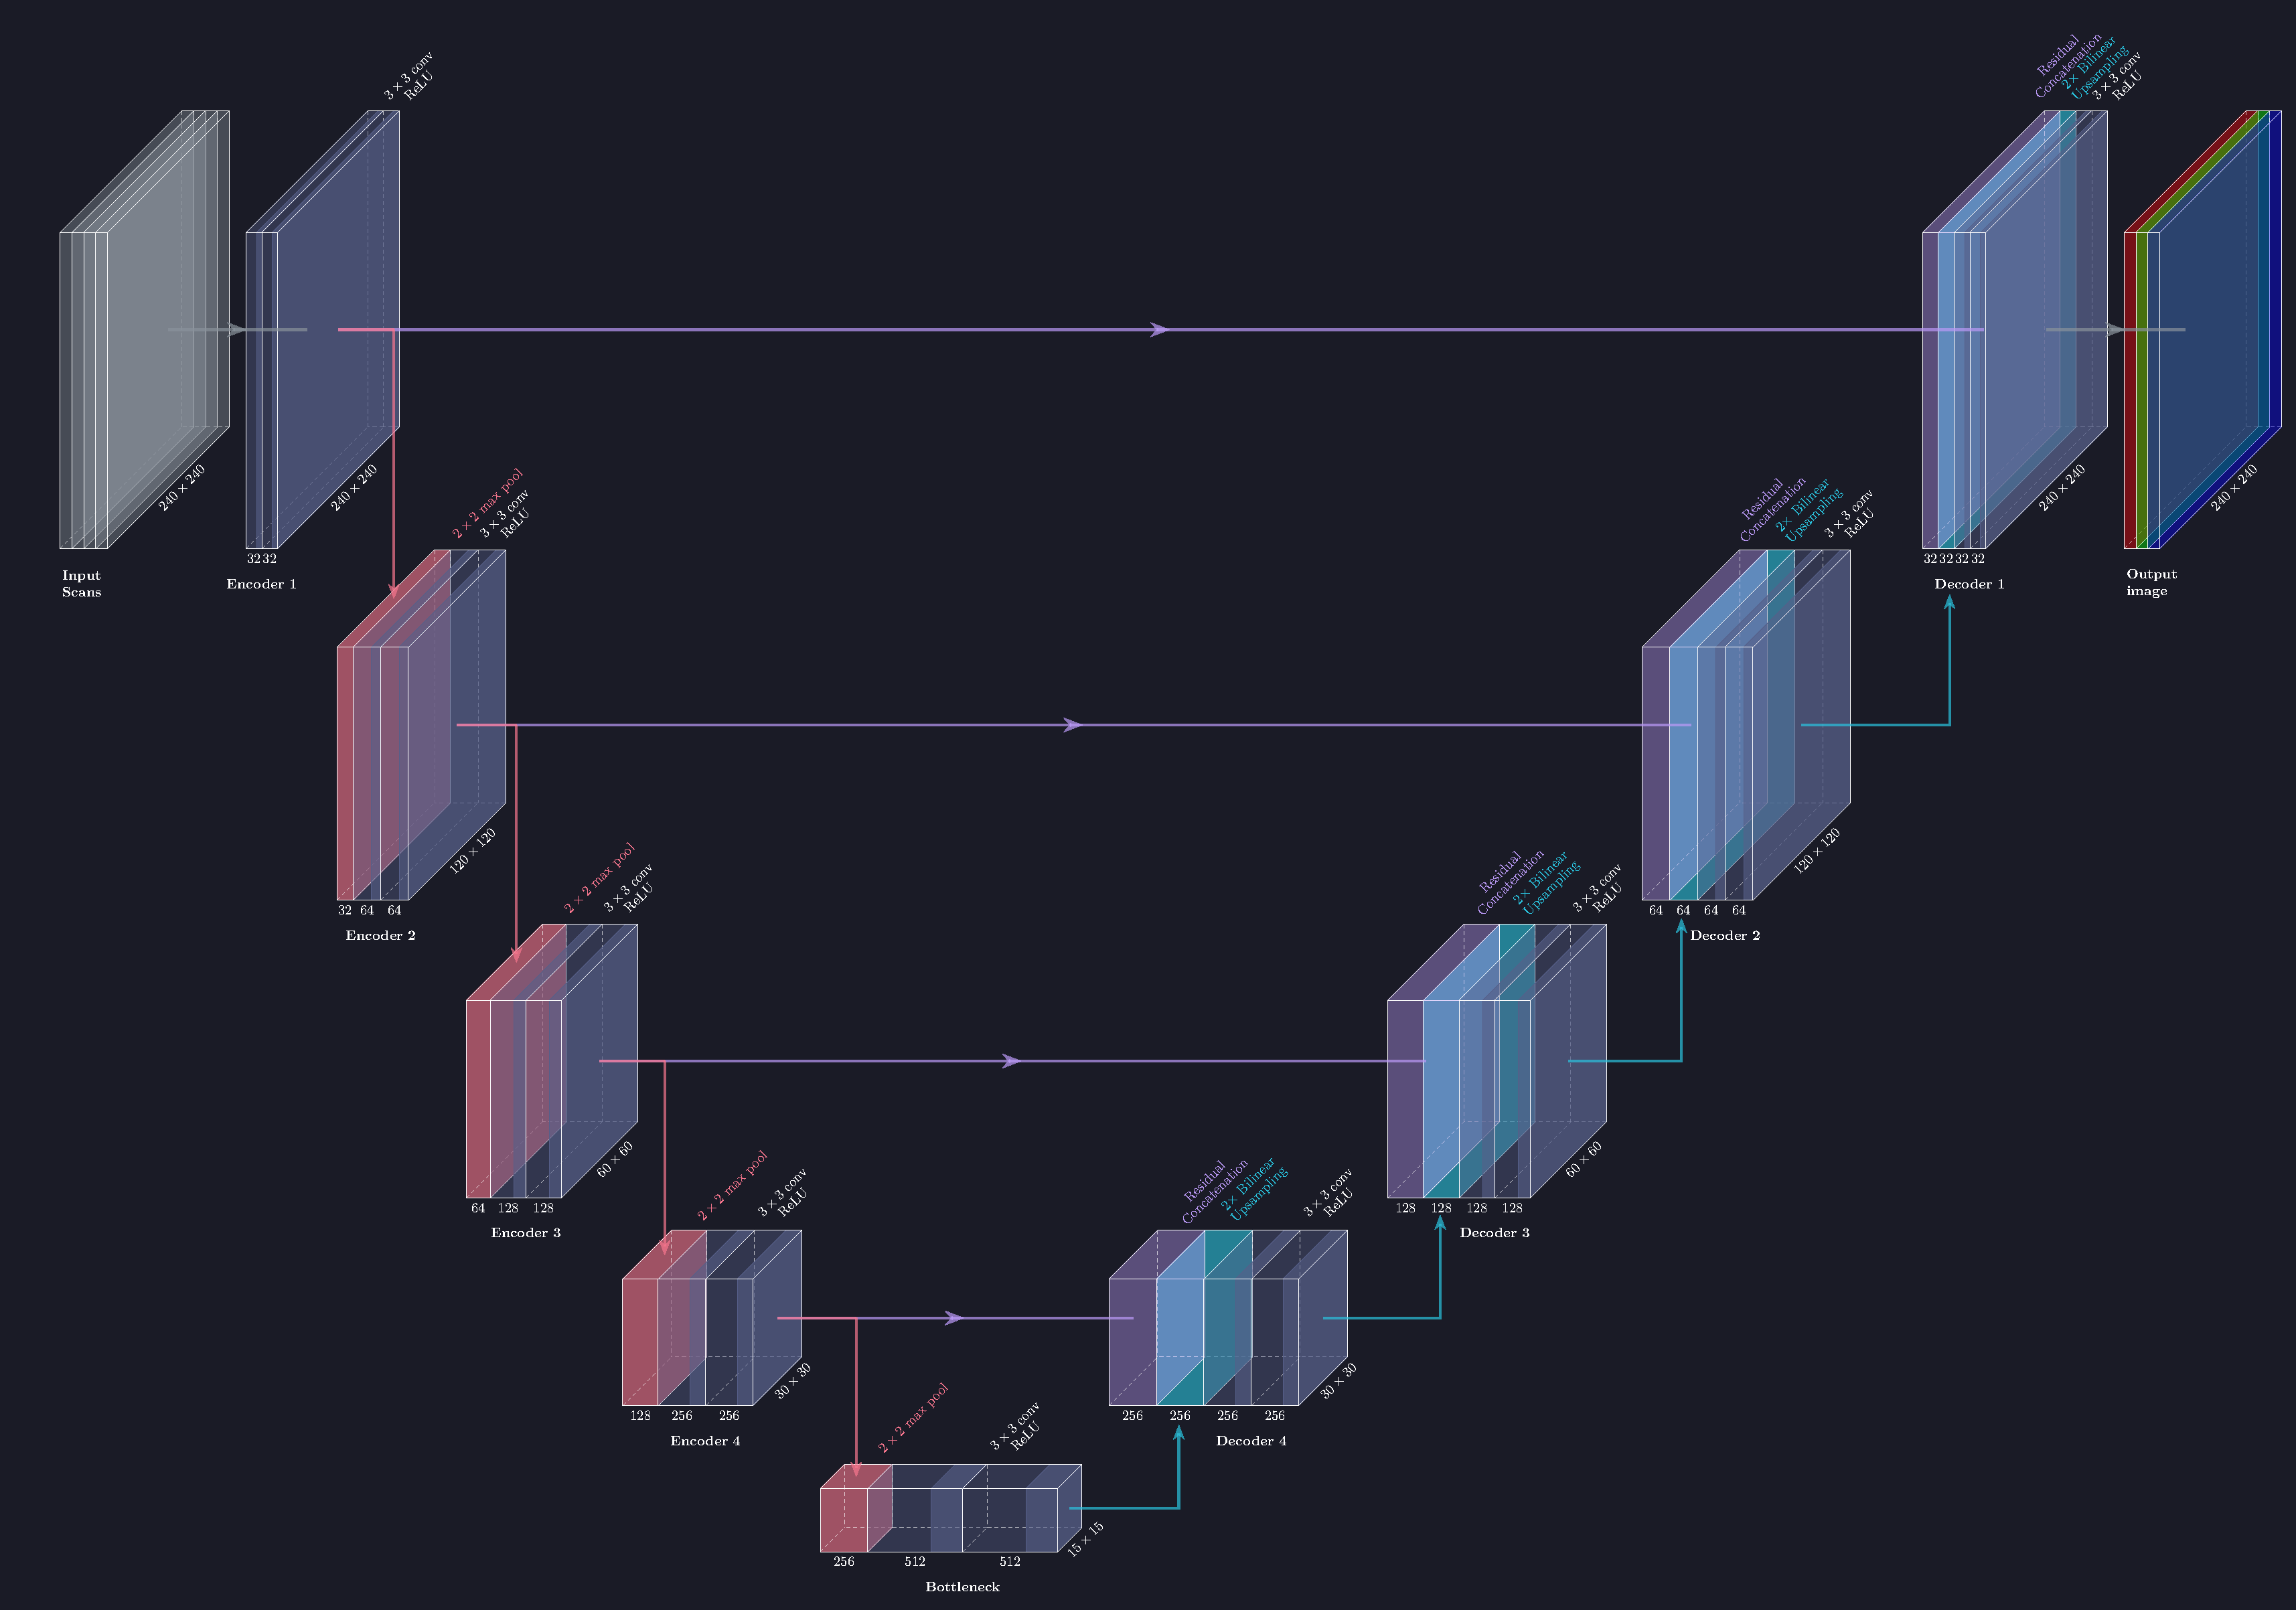
\includegraphics[width=\textwidth]{classic-unet-5.pdf}}
			};
			% Adjust the position of the text
			\node[align=center] at ($(current page.center) + (0, 2.5)$) {
				\only<1>{Input: $4$ channels \quad Output: $3$ channel}%
				\only<2>{\yellow{$3 \times 3$ convolutions $+$ ReLU activations}}%
				\only<3>{\red{$2 \times 2$ Max pooling}}%
				\only<4>{\azure{$2 \times$ Bilinear upsampling}}%
				\only<5>{\purple{Skip connections: concatenation}}
			};
	\end{tikzpicture}

\end{frame}


% Slide 3 ──────────────────────────────────────────────────────────────────────
\begin{frame}[t]

	\frametitle{Improved U-Net}

	% Small improvements from previous $\rightarrow$ to reduce $n^{\circ}$ of
	% parameters and improve performance:

	% \vspace{4ex}

	% \begin{itemize}
	% 	 \setlength{\itemsep}{4ex}
	% 	\item \bft{Separable Convolutions}: \gray{depthwise $+$ pointwise
	% 		convolutions} 
	% 	\item \bft{Batch Normalization}: \gray{to improve training and
	% 		generalization}
	% 	\item \bft{Larger Kernel Size}: \gray{$7 \times 7$ kernels instead of $3
	% 		\times 3$}
	% 	\item \bft{Inverse Bottleneck}: \gray{expands $+$ compresses channels}
	% 	\item \bft{Additive Skip Connections}: \gray{instead of concatenated ones}
	% \end{itemize}

	\centering

	\begin{tikzpicture}[remember picture,overlay]
			% Adjust the position of the image
			\node[anchor=south] at ($(current page.south) + (0, 0.4)$) {
				\only<1>{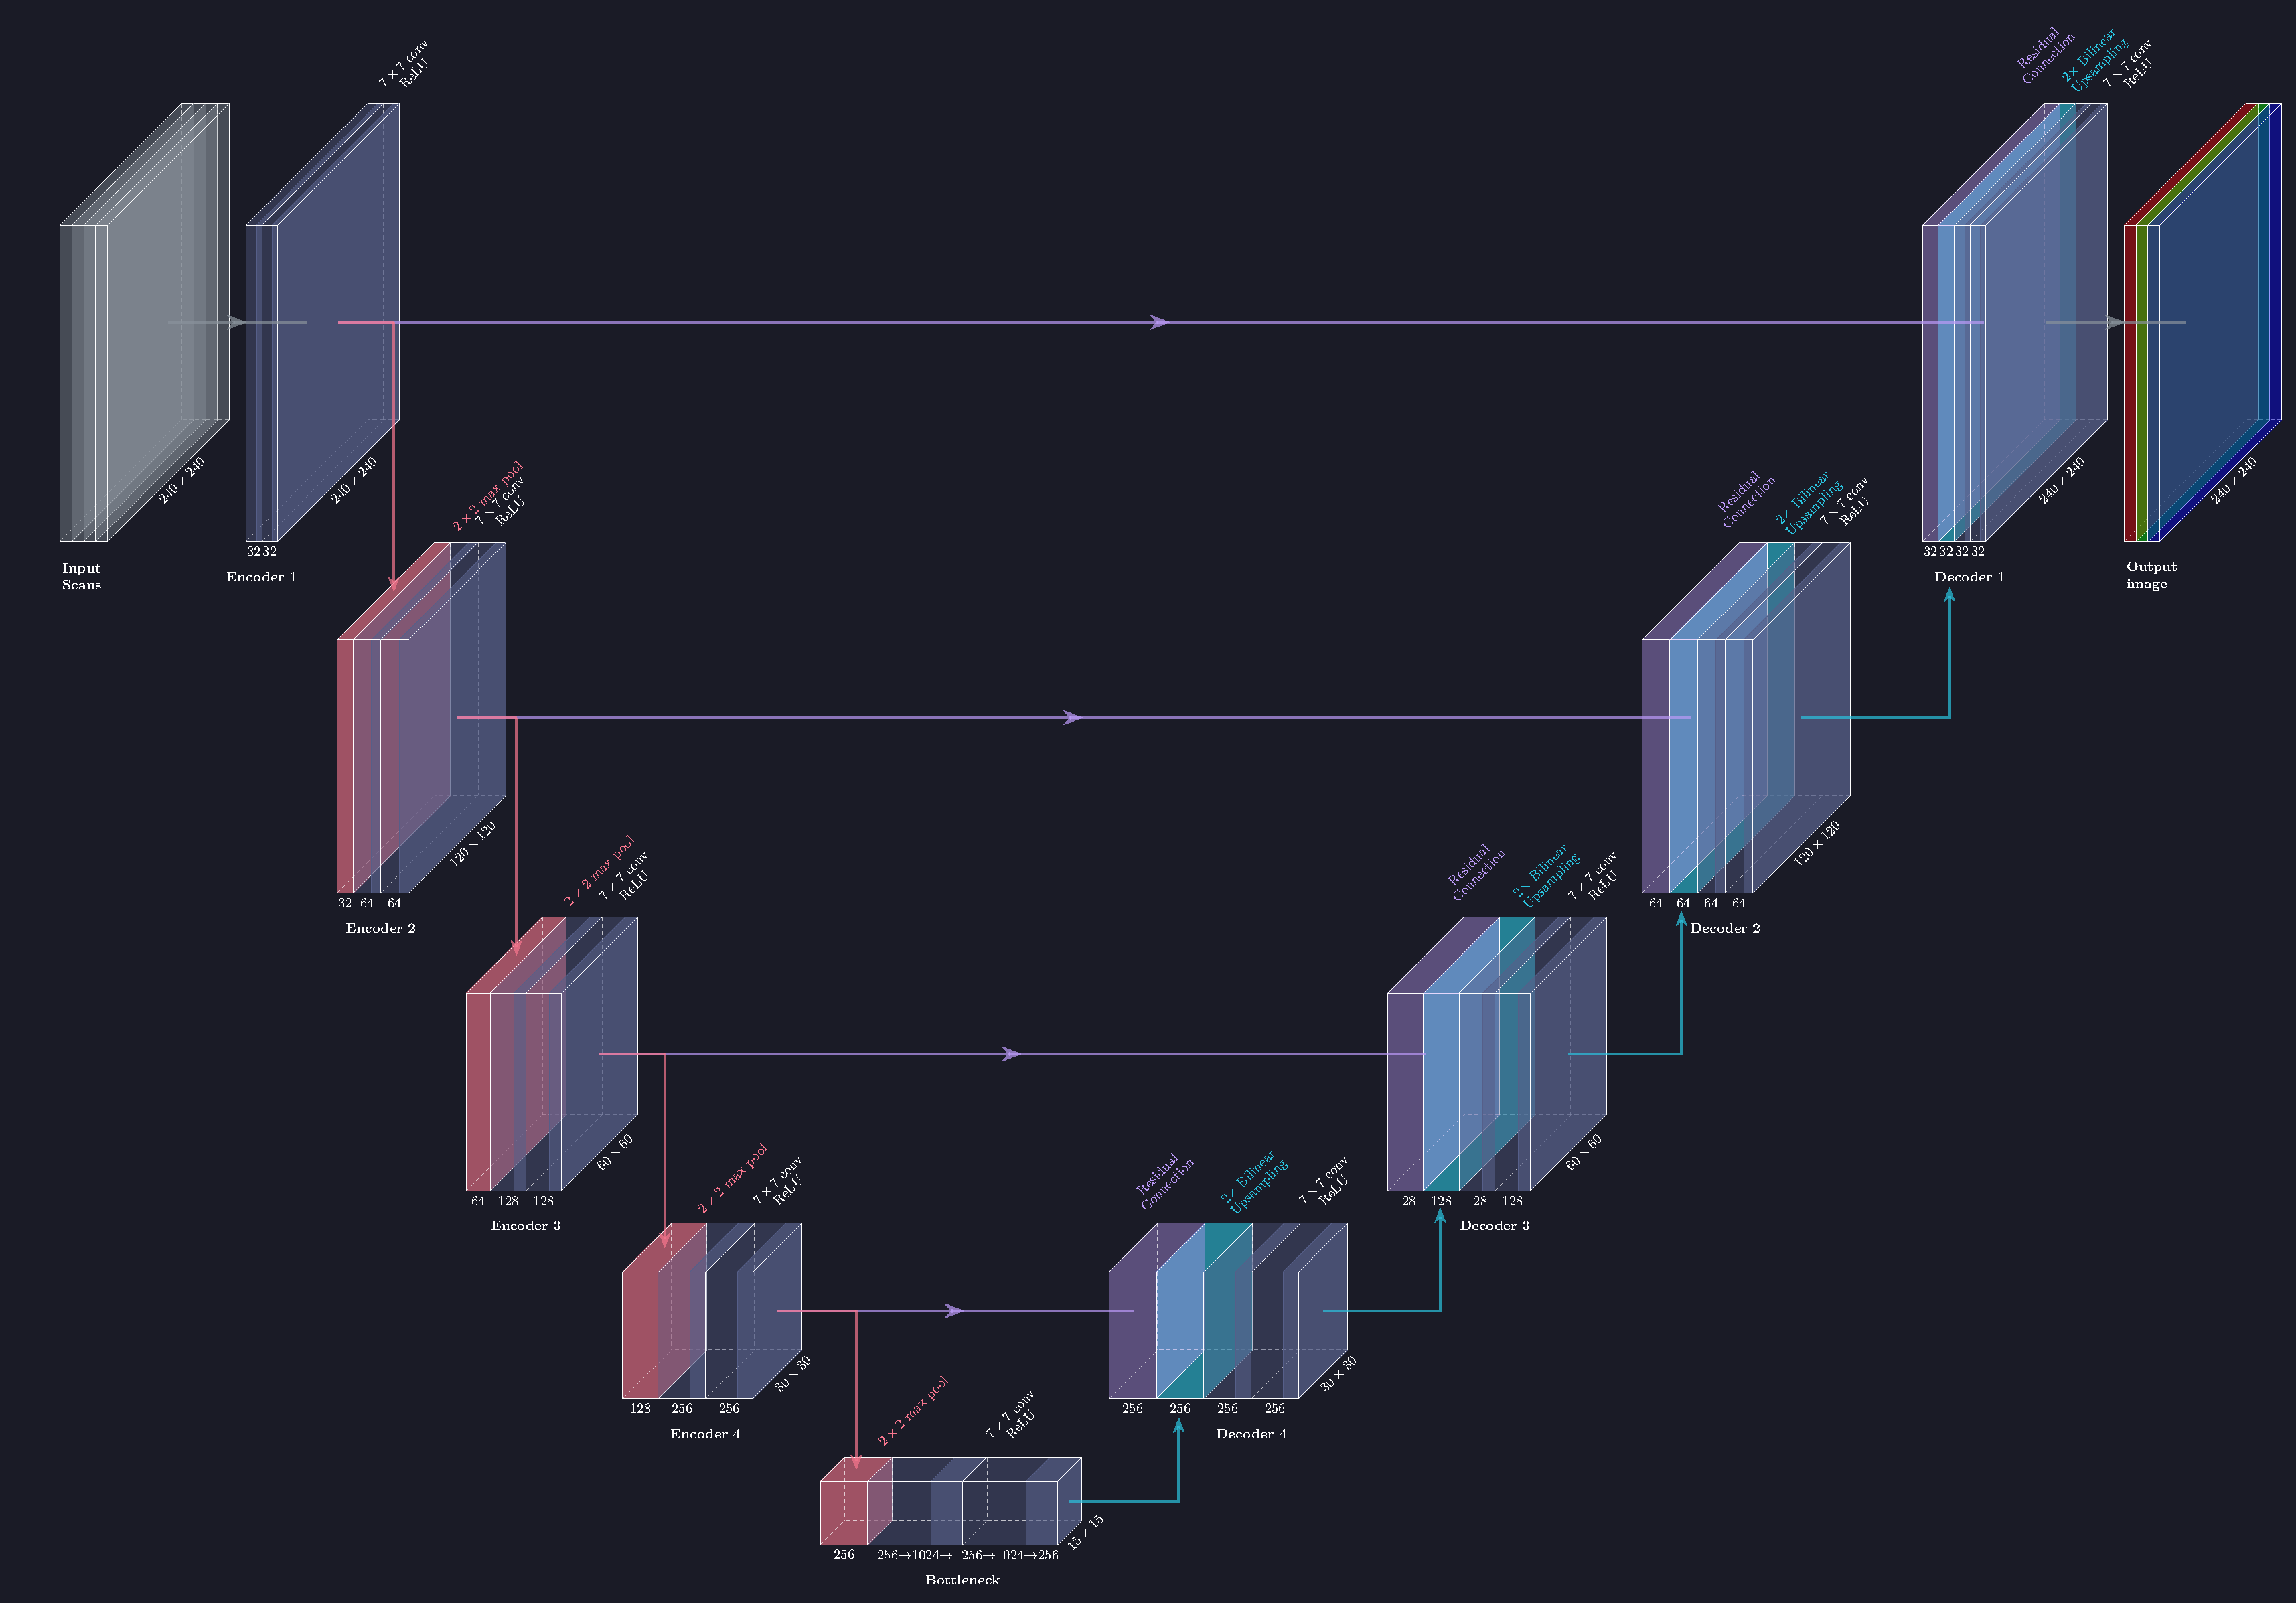
\includegraphics[width=\textwidth]{improved-unet-1.pdf}}%
				\only<2>{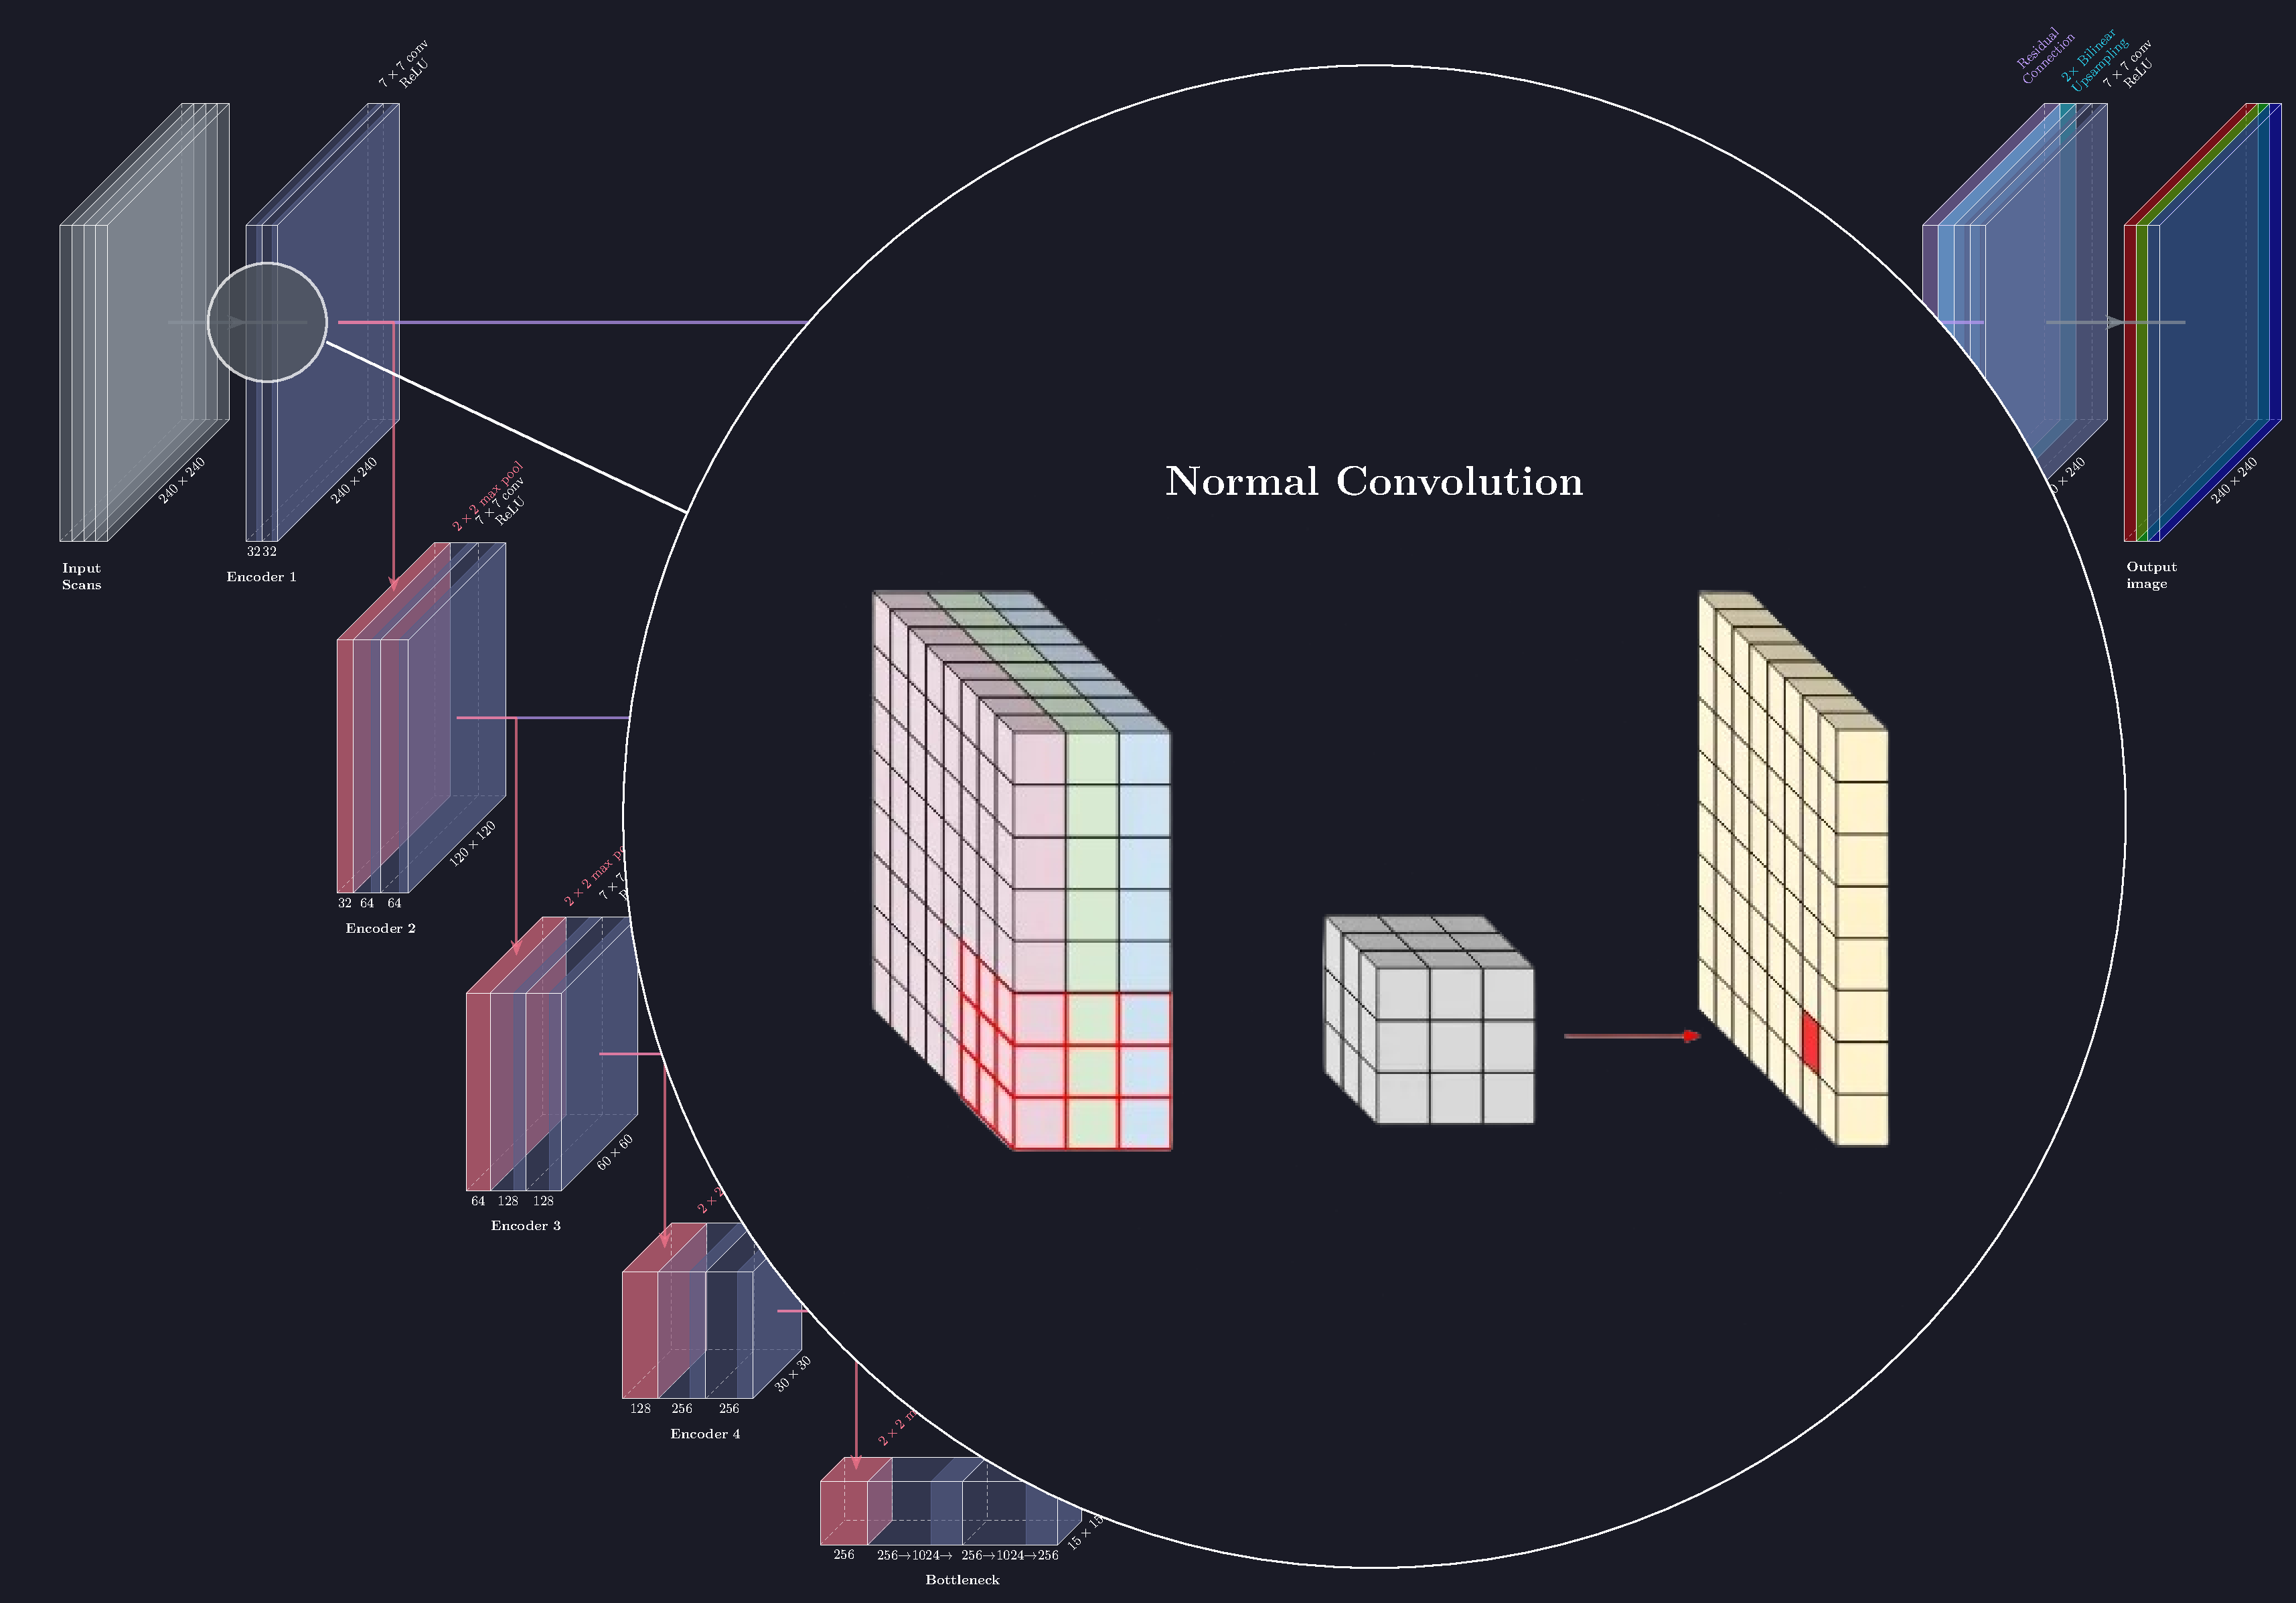
\includegraphics[width=\textwidth]{improved-unet-zoom1.pdf}}%
				\only<3>{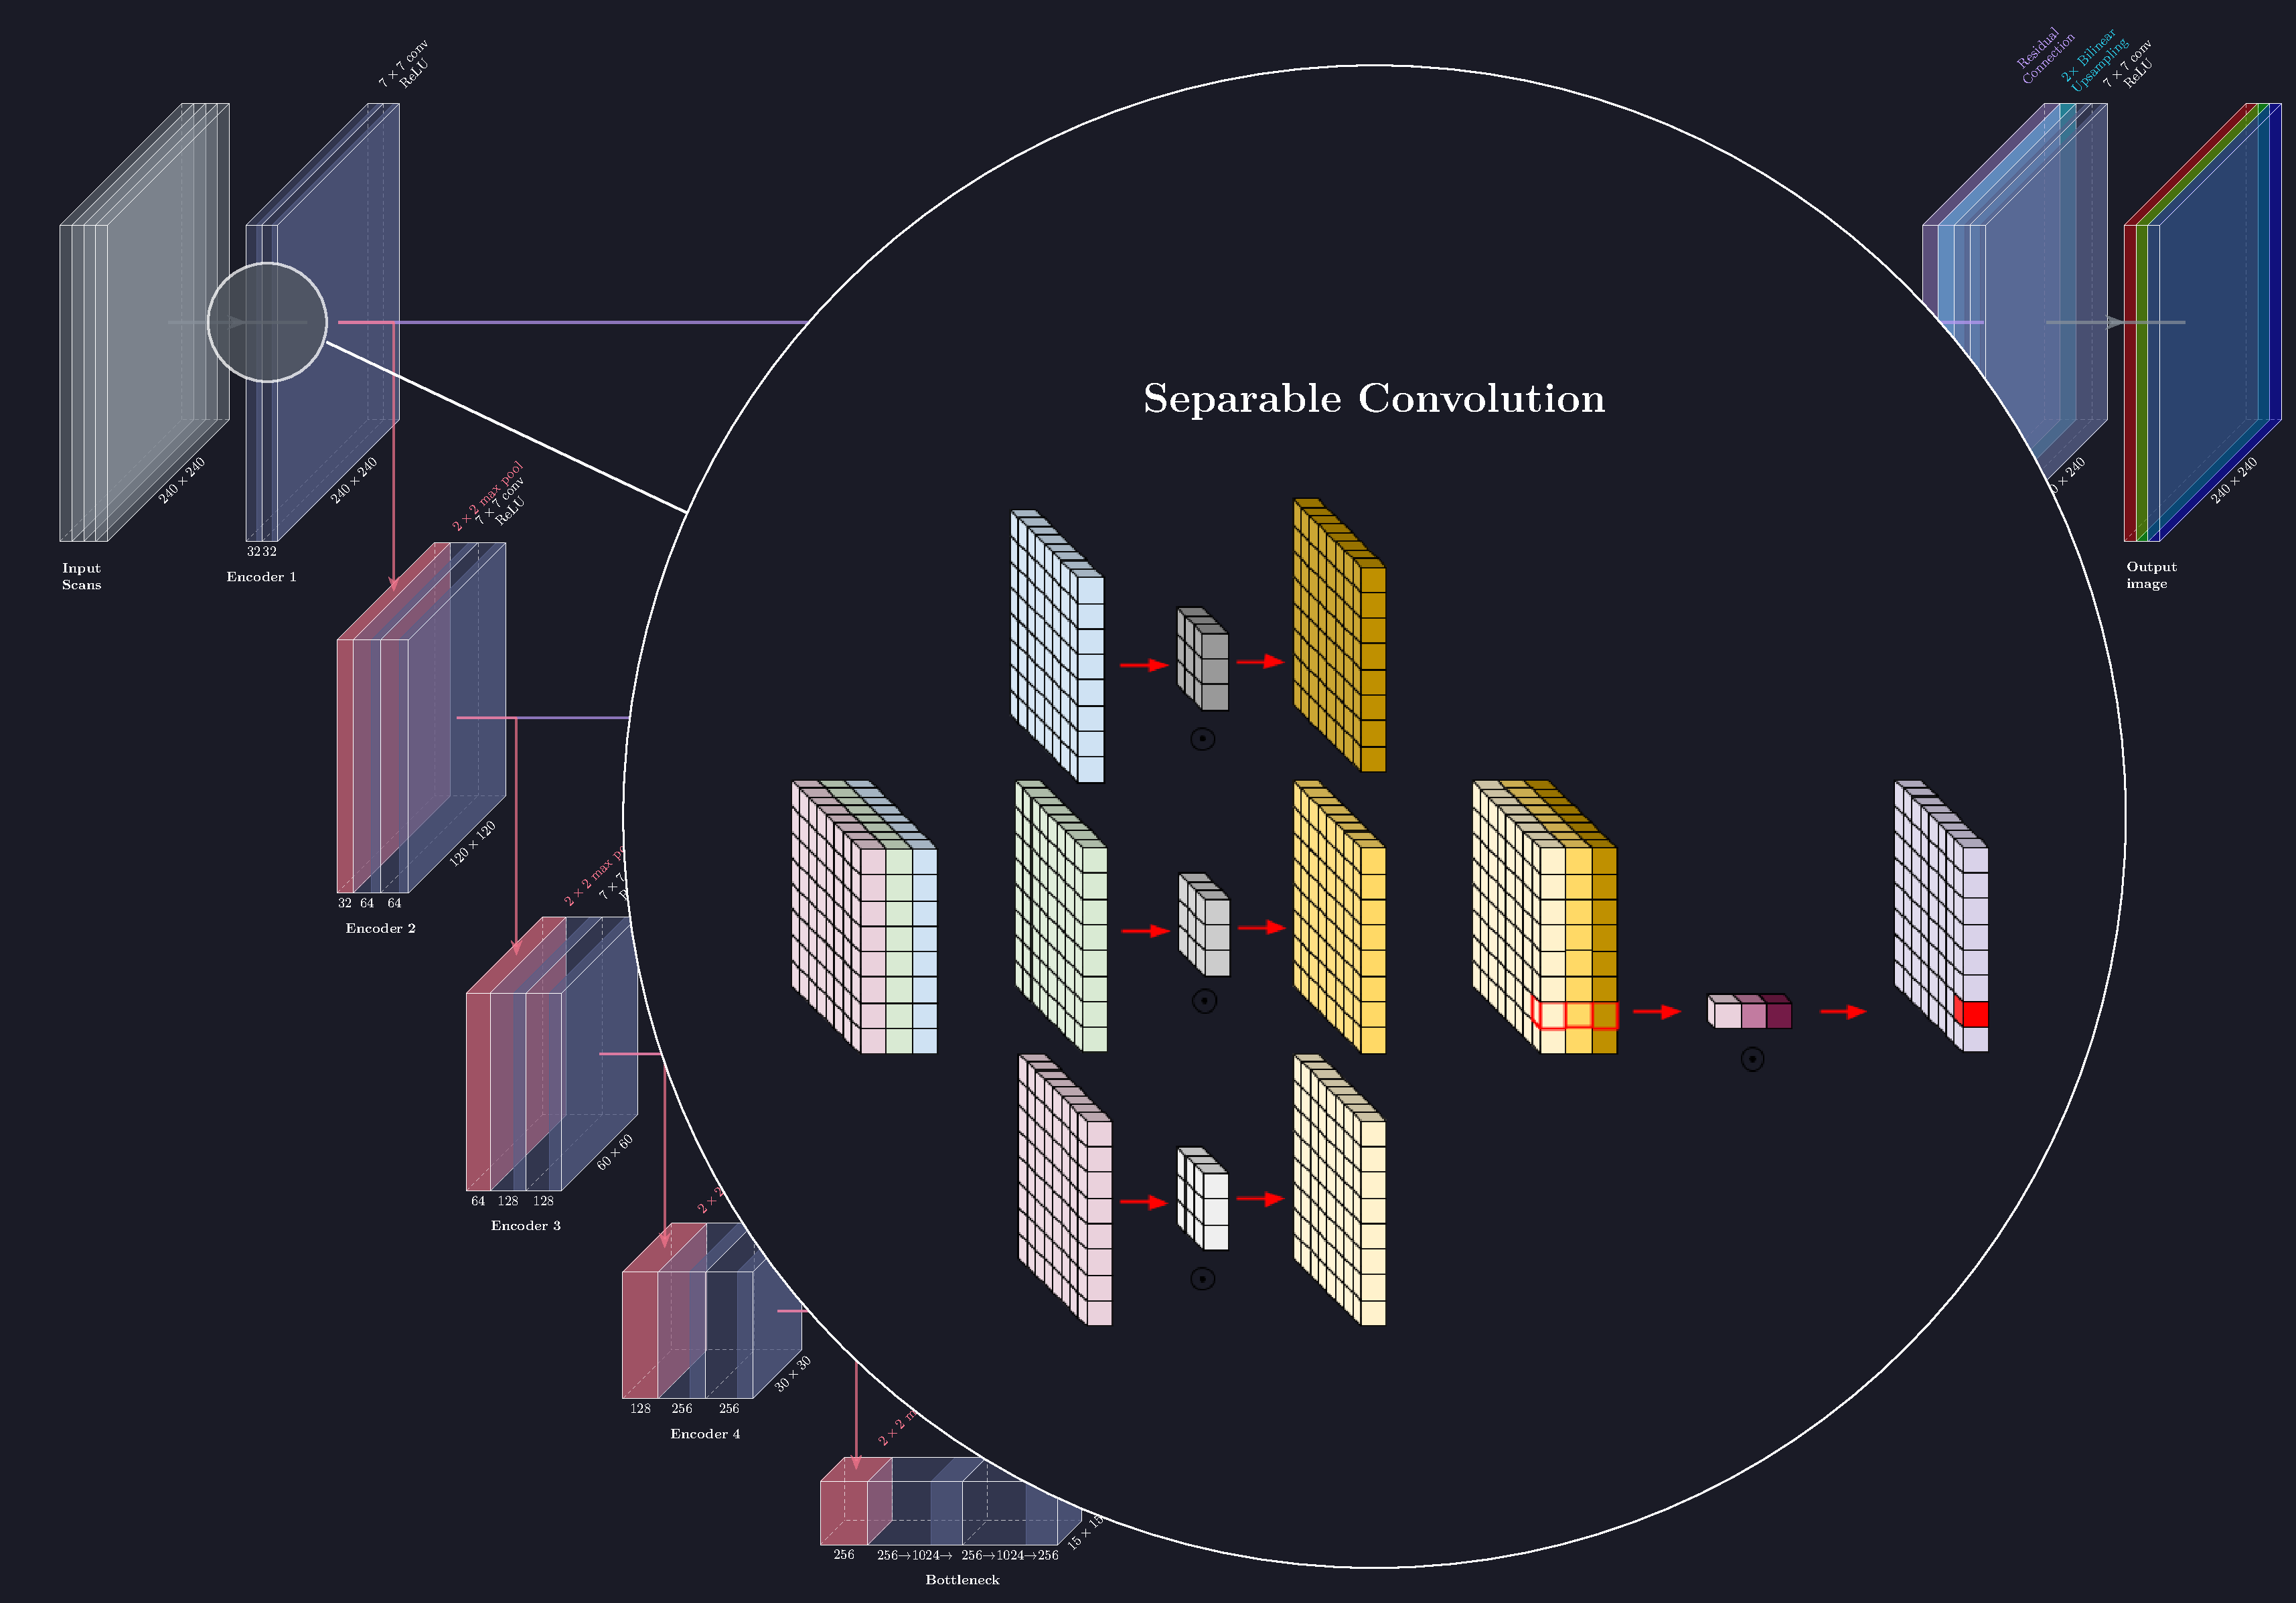
\includegraphics[width=\textwidth]{improved-unet-zoom2.pdf}}%
				\only<4>{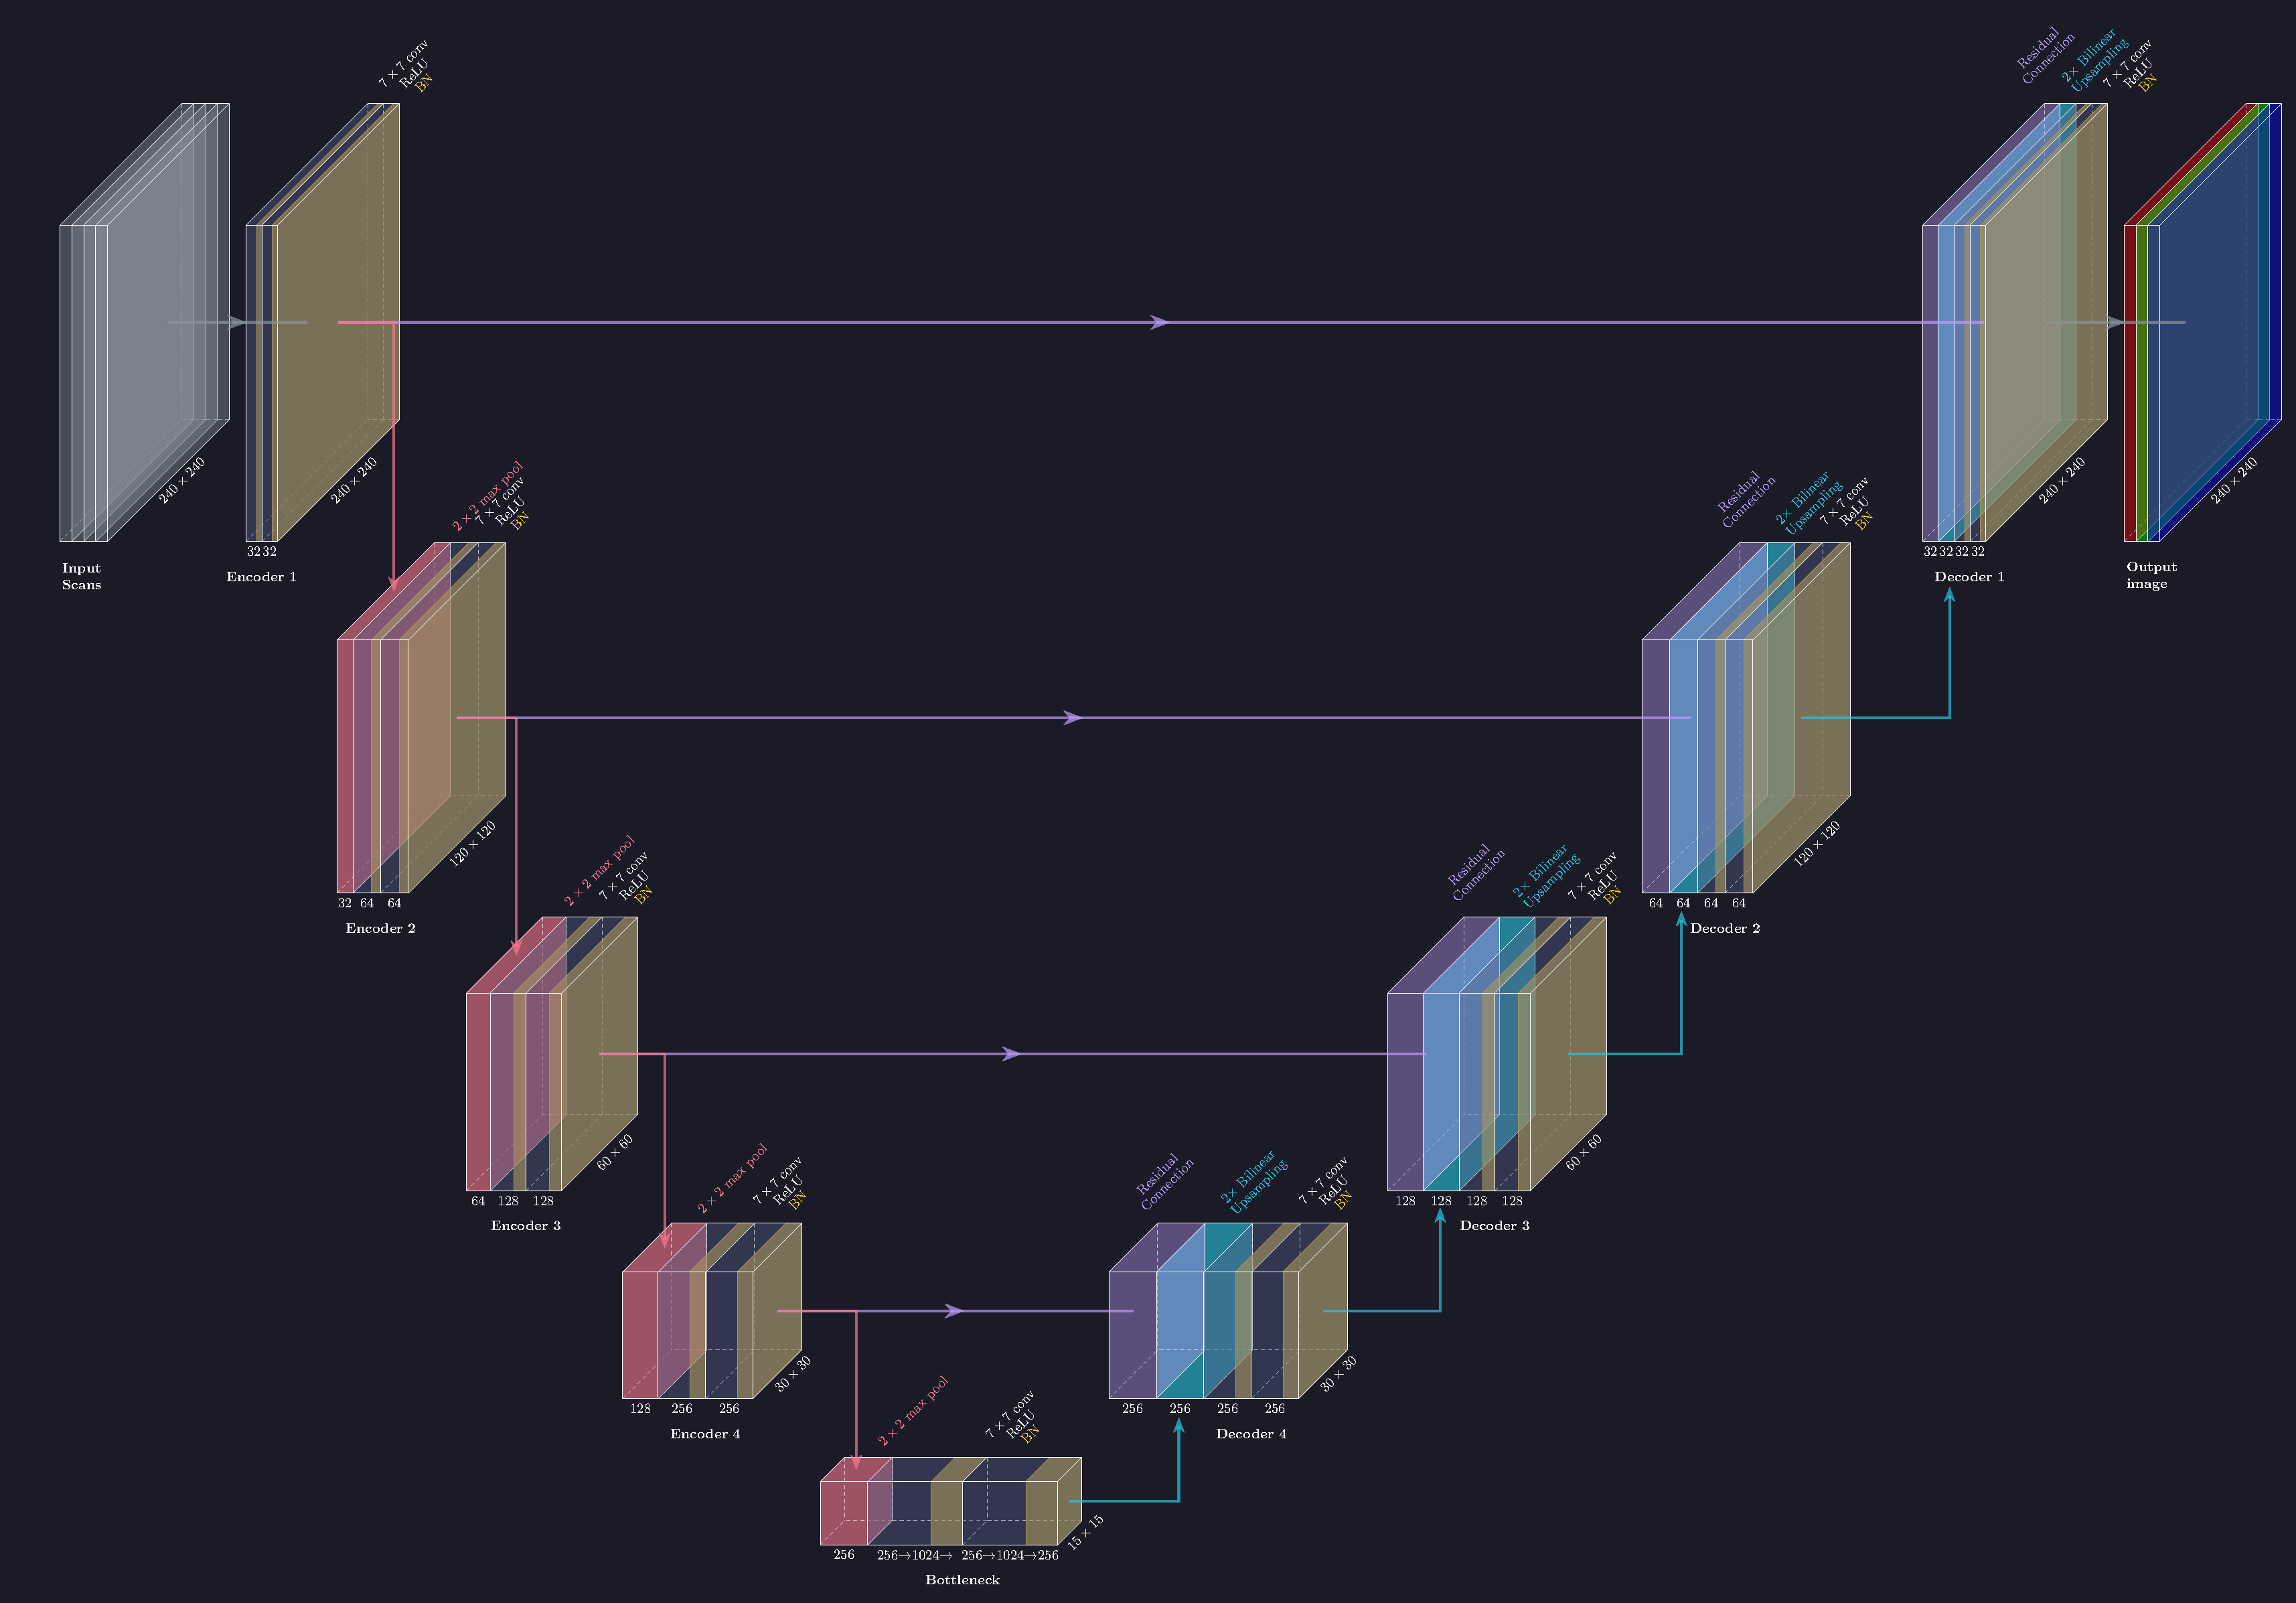
\includegraphics[width=\textwidth]{improved-unet-2.pdf}}%
				\only<5>{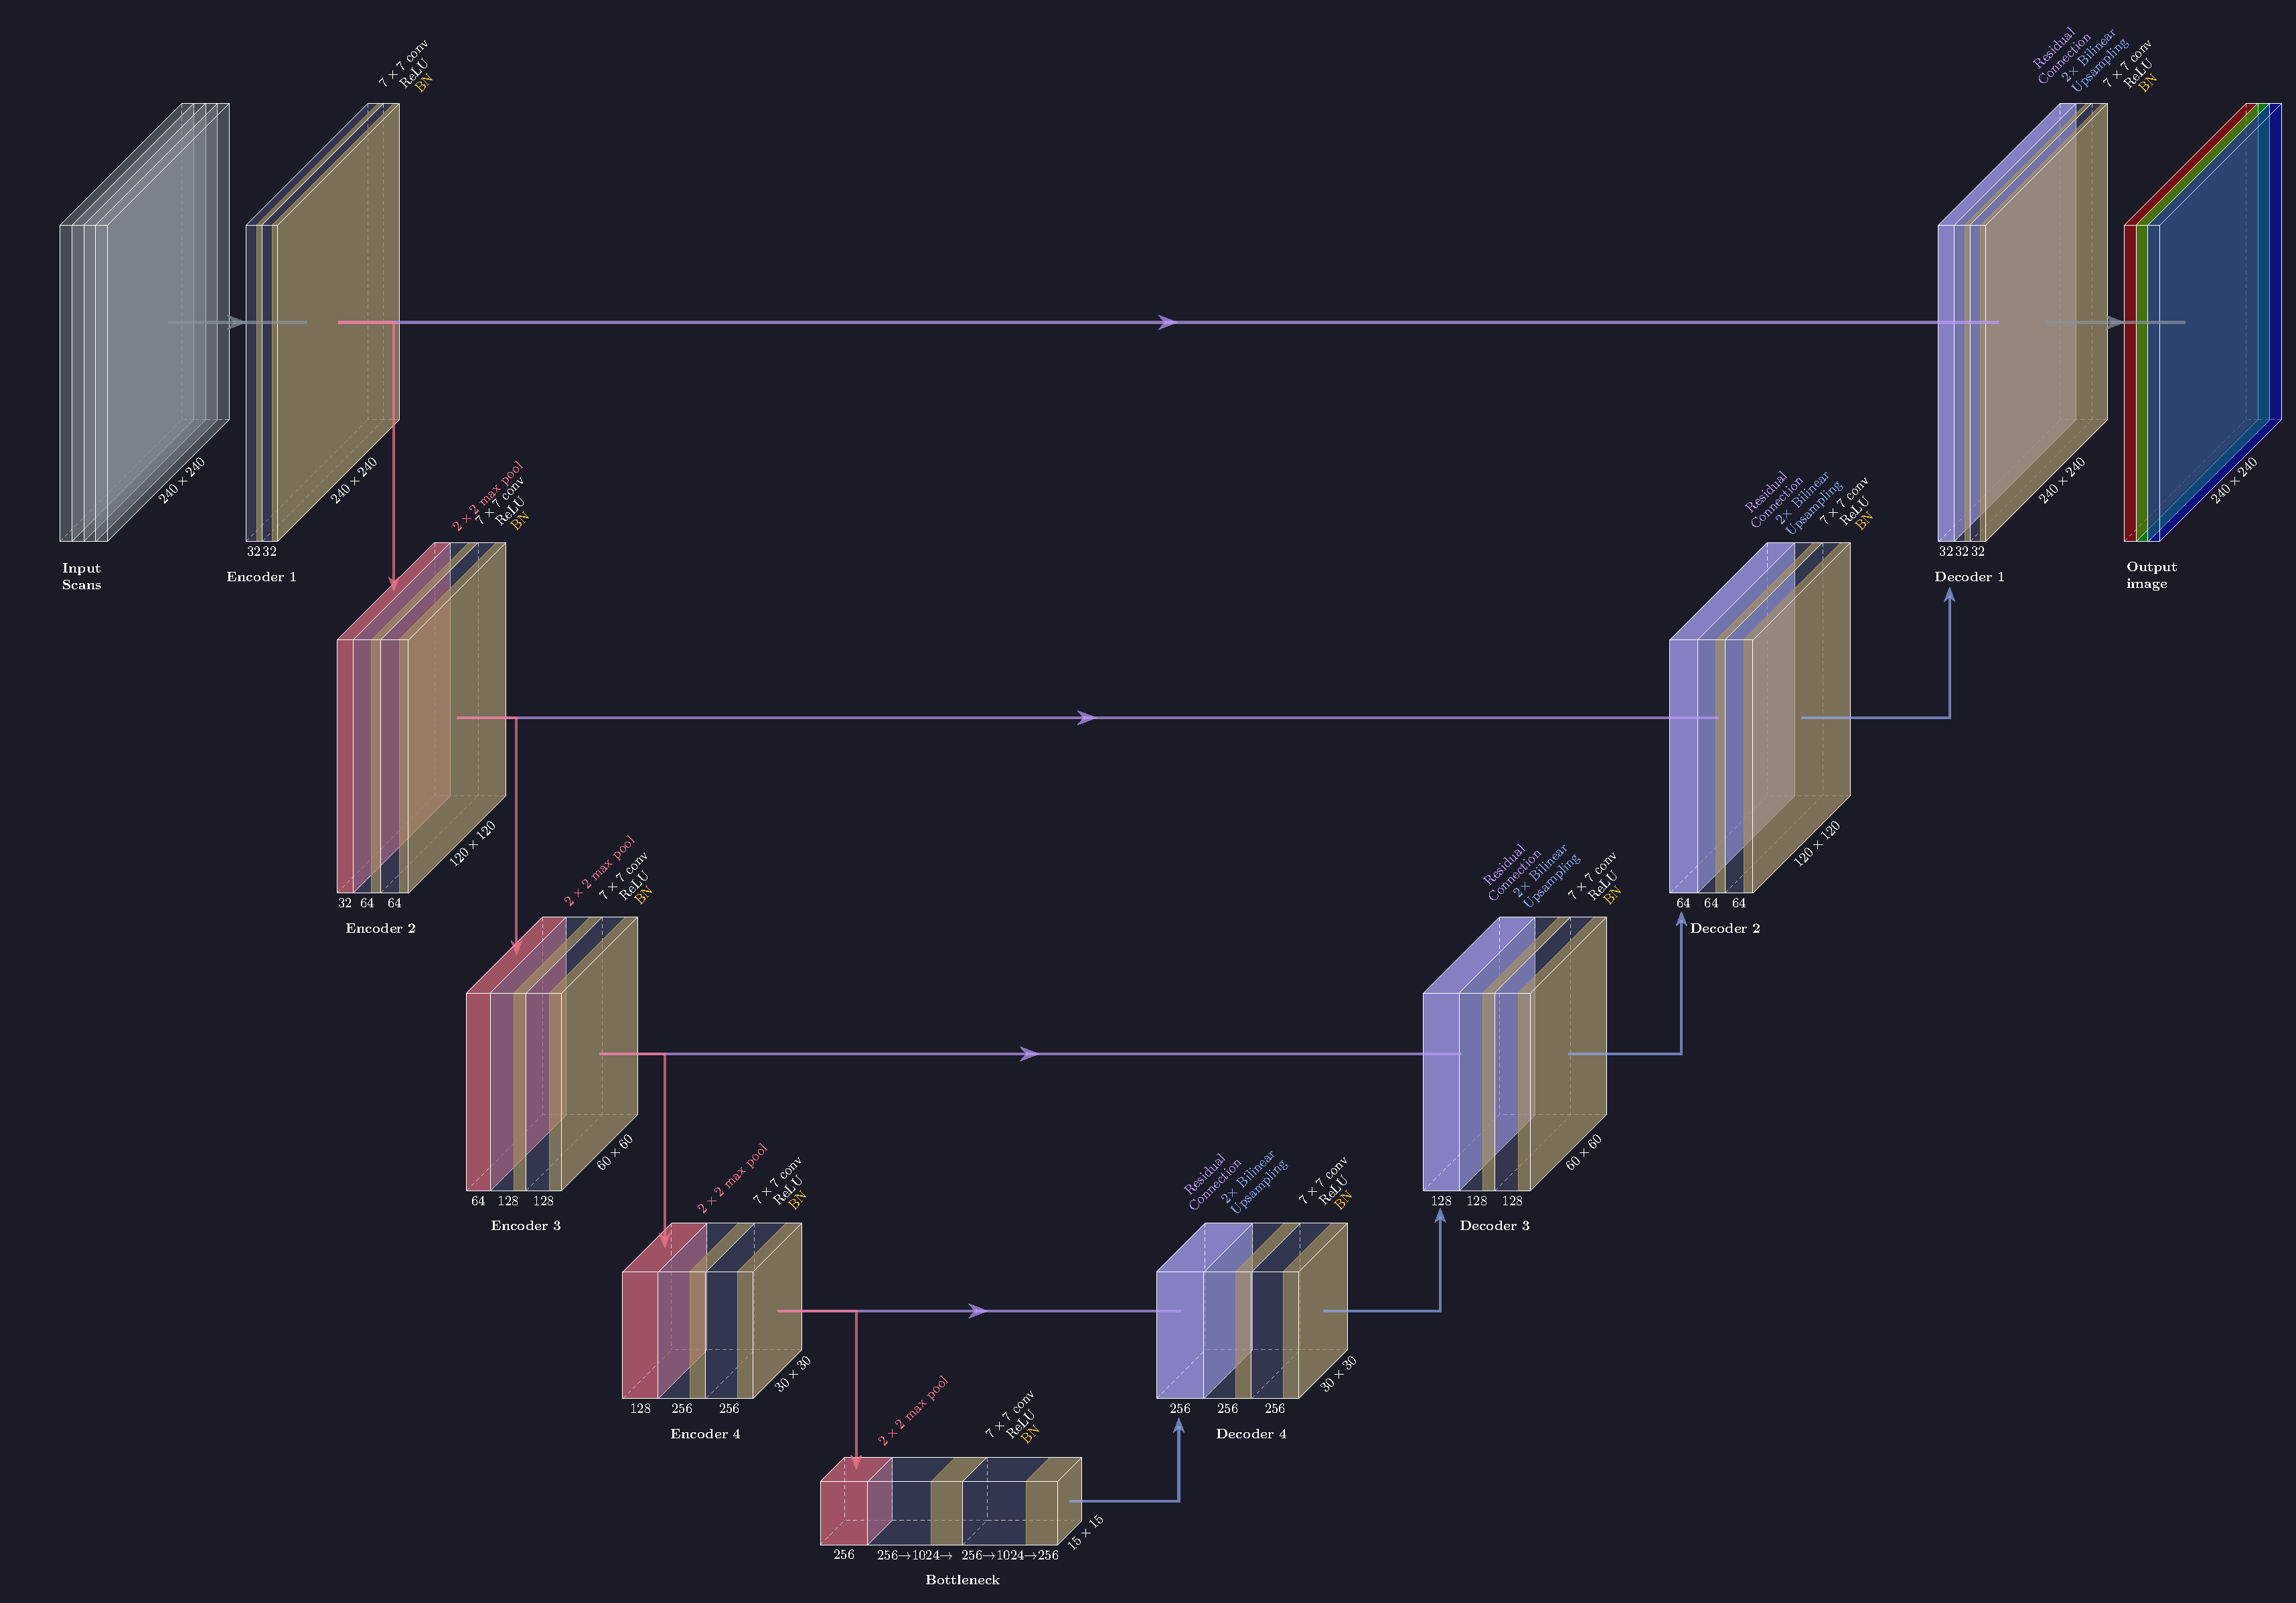
\includegraphics[width=\textwidth]{improved-unet-3.pdf}}%
			};
			% Adjust the position of the text
			\node[align=center] at ($(current page.center) + (0, 2.5)$) {
				\only<1>{Separable Convolutions \\ $7 \times 7$ kernels \\ Inverse
				Bottleneck}%
				\only<4>{\yellow{Batch Normalization}}%
				\only<5>{\purple{Additive skip connections}}
			};
	\end{tikzpicture}

\end{frame}


% Slide 4 ──────────────────────────────────────────────────────────────────────
\begin{frame}[t]

	\frametitle{Attention U-Net}

	\begin{tikzpicture}[remember picture,overlay]
			\node[anchor=south] at ($(current page.south) + (0, 0.4)$) {
				\only<1>{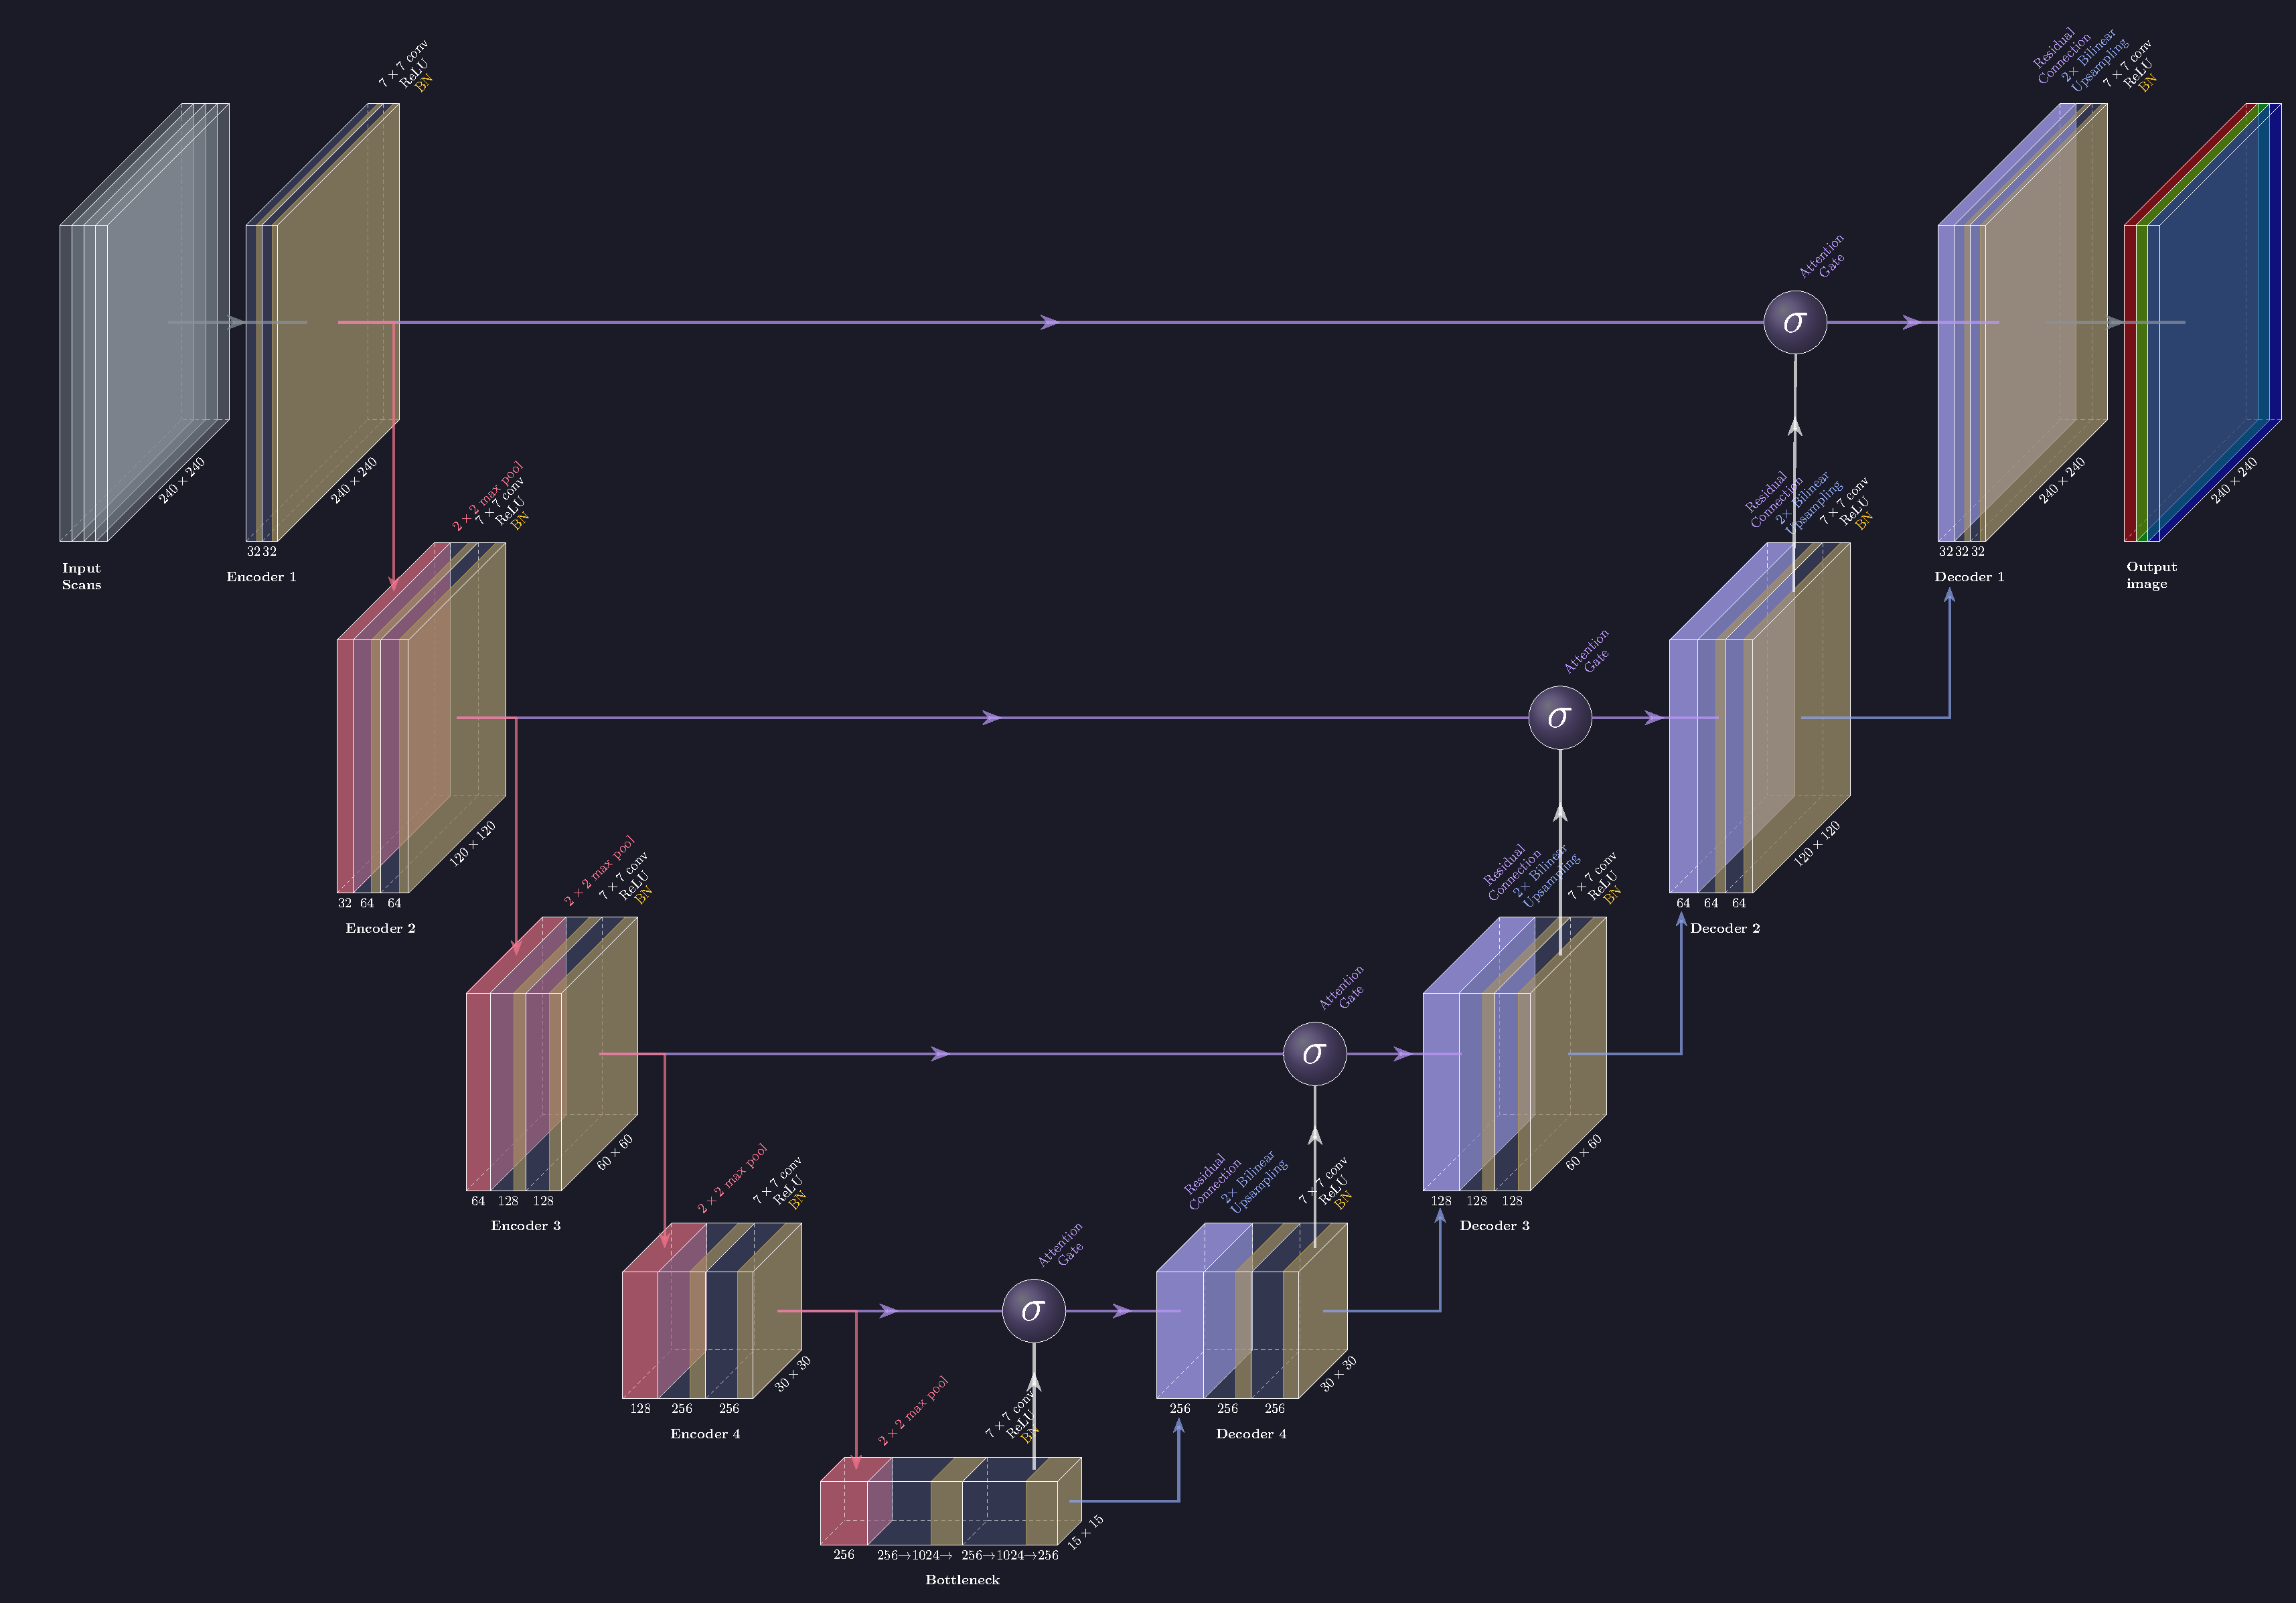
\includegraphics[width=\textwidth]{attention-unet.pdf}}%
				\only<2>{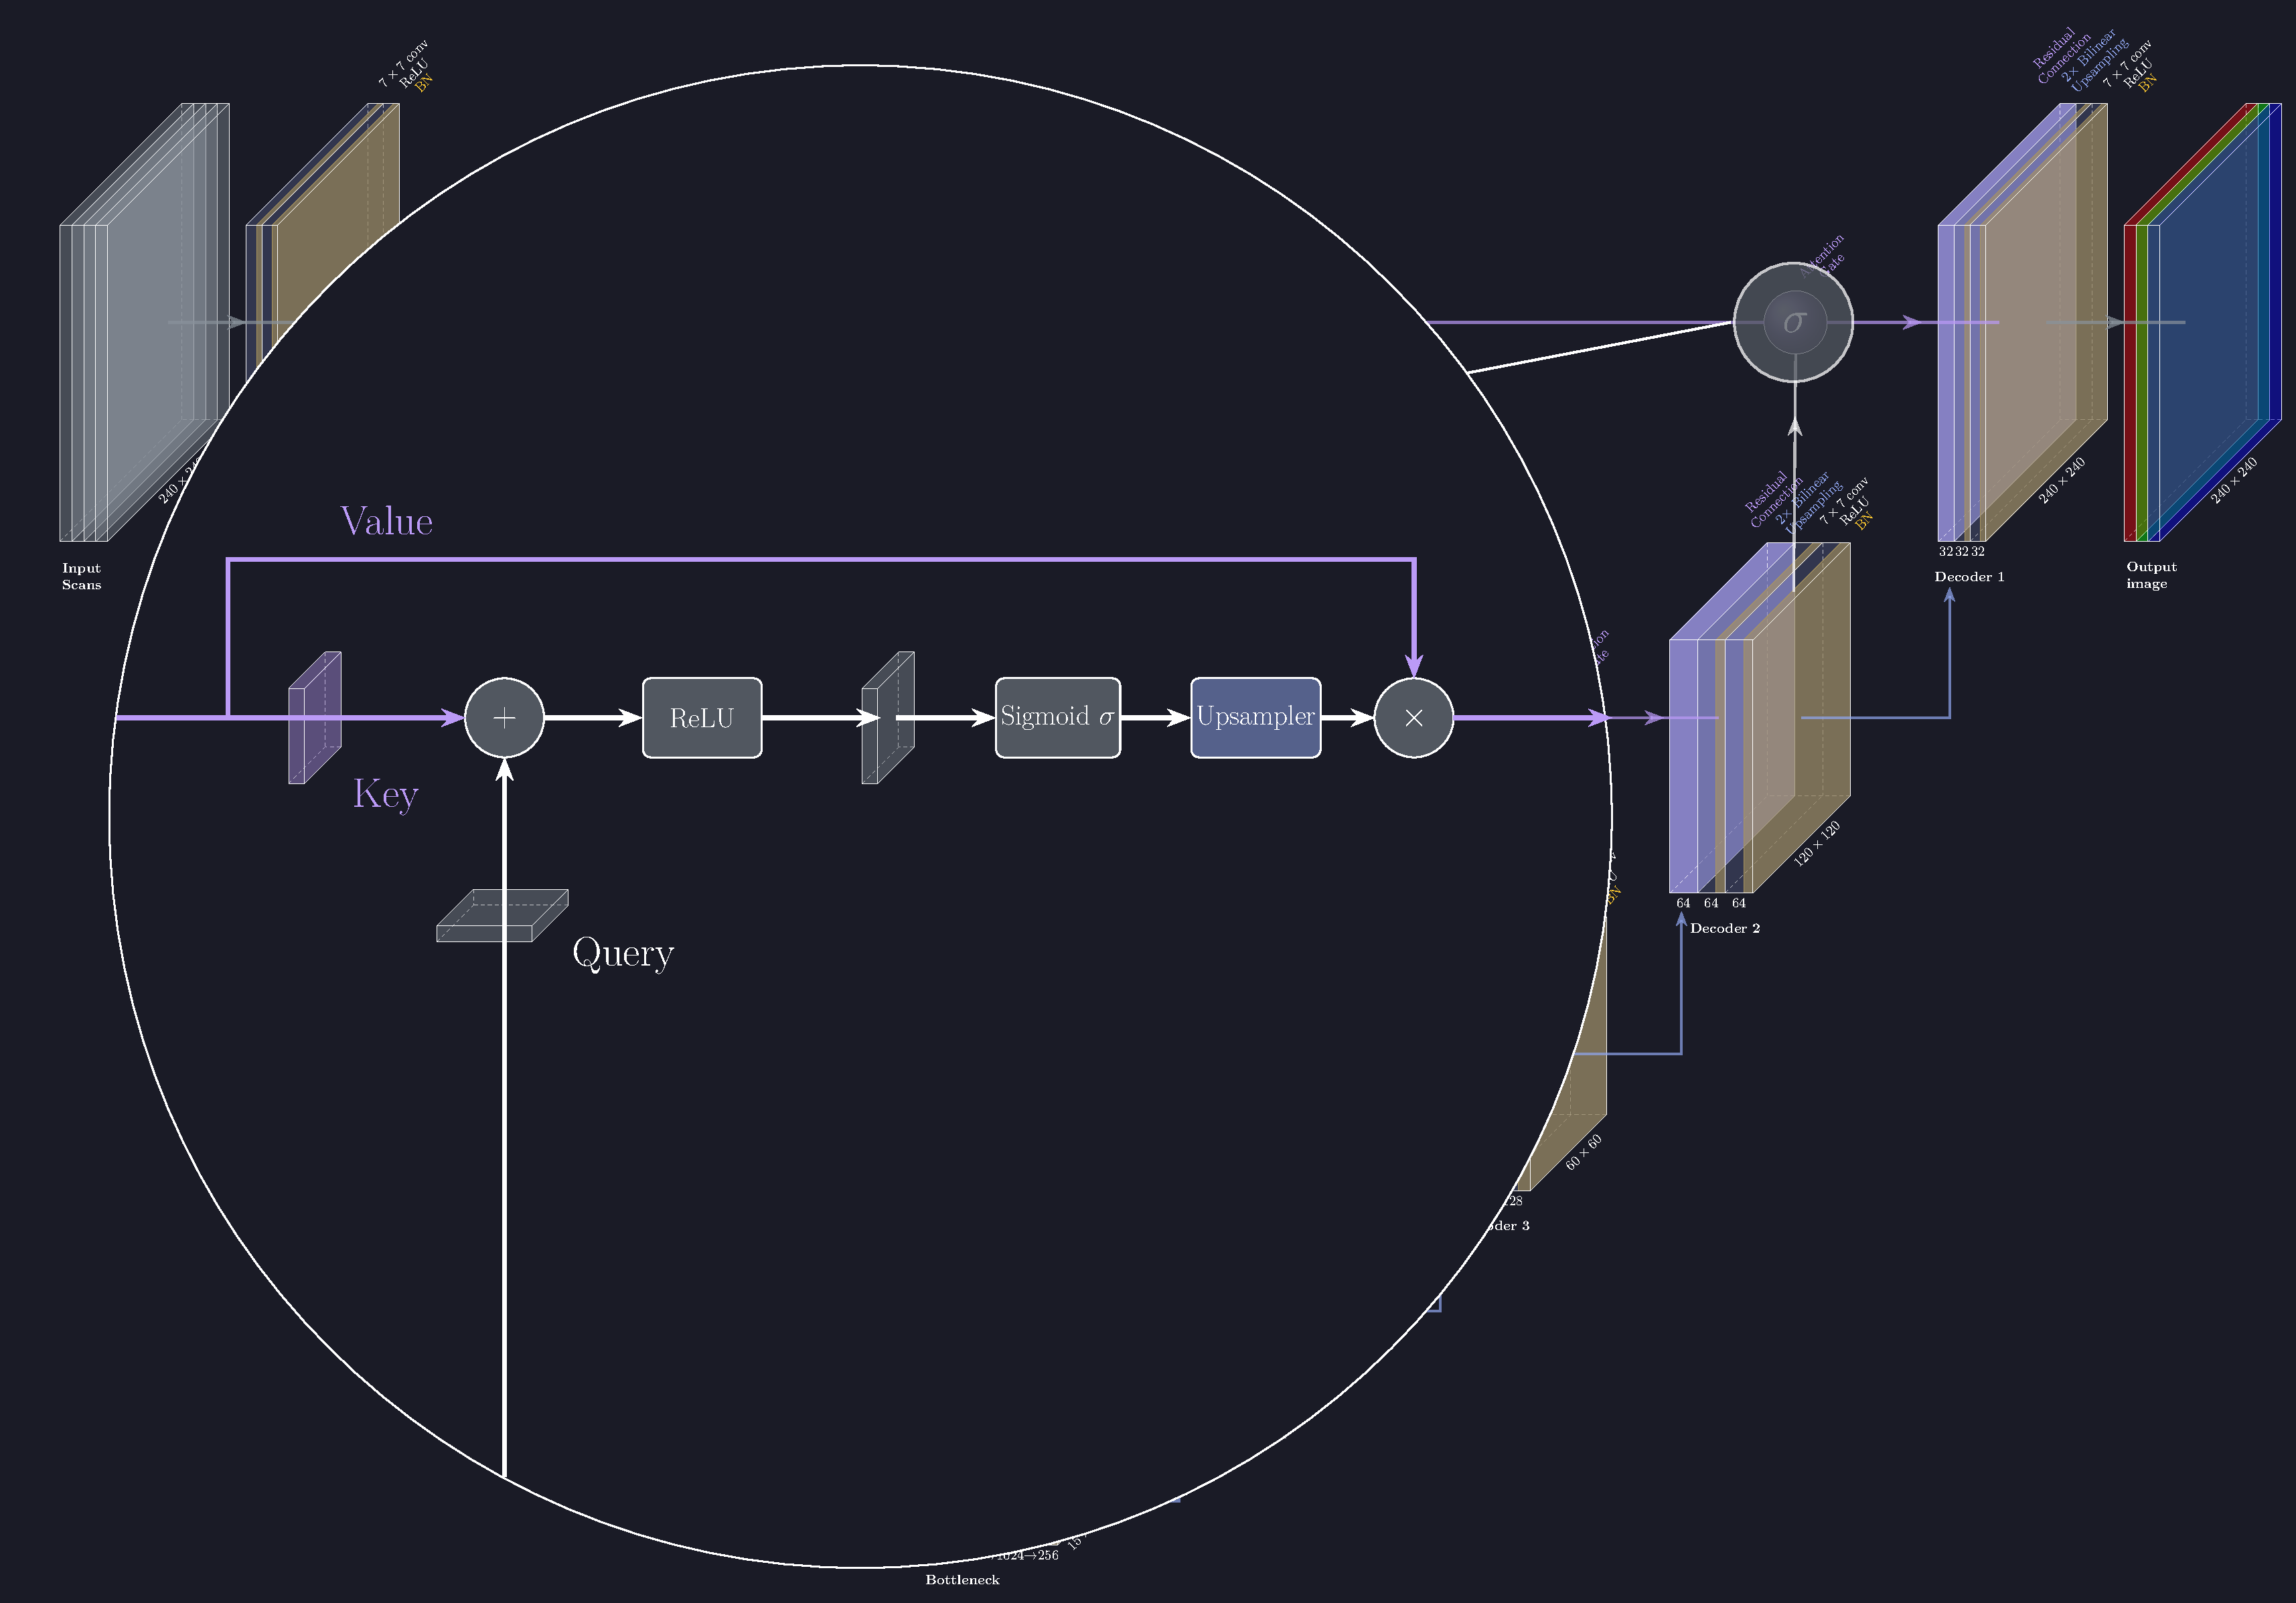
\includegraphics[width=\textwidth]{attention-unet-zoom.pdf}}
			};
	\end{tikzpicture}

\end{frame}


% Slide 5 ──────────────────────────────────────────────────────────────────────
\begin{frame}[t]

	\frametitle{Training Details}

	U-Net models training parameters:
	\vspace{0.2cm}

	\begin{itemize}
		\setlength{\itemsep}{1.5ex}
		\item \bft{Epochs}: $20$
		\item \bft{Optimizer}: Adam \gray{(with weight decay $1 \times 10^{-2}$)}
		\item \bft{Scheduler}: Exponential Decay \gray{($\gamma = 0.9$)}
		\item \bft{Loss function}: BCE with Logits Loss:
			\begin{equation*}
				\ell(y, \hat{y}) = - \left[ 
					y \log(\sigma(\hat{y})) + (1 - y) \log(1 - \sigma(\hat{y}))
				\right]
			\end{equation*}
		\item \bft{Learning rate}: $2 \times 10^{-3}$
		\item \bft{Batch size}: $32$ \gray{(both training and validation)}
		\item \bft{First encoder filters}: $32$
		\item \bft{Image size}: $240 \times 240$
	\end{itemize}

\end{frame}


% Slide 6 ──────────────────────────────────────────────────────────────────────
\begin{frame}

	\frametitle{Visualizing a prediction}

	\vspace{-2ex}

		\begin{figure}
			\centering
			\only<1>{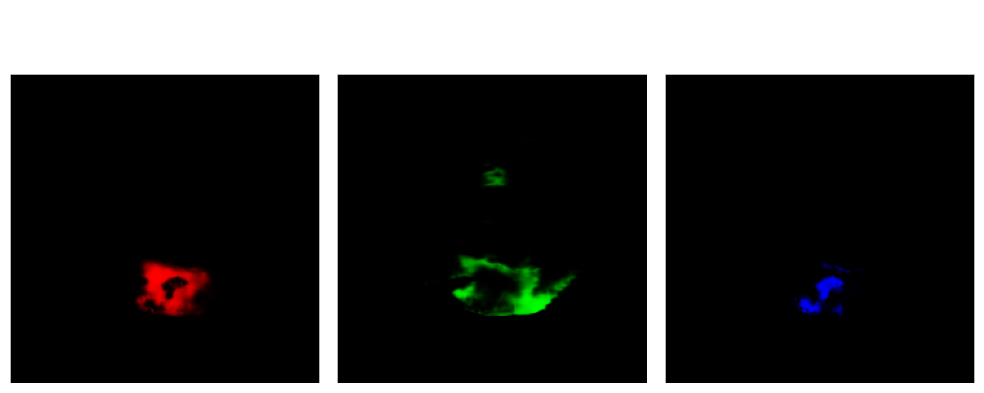
\includegraphics[width=0.85\textwidth]{segmentation-prediction.png}}
			\only<2->{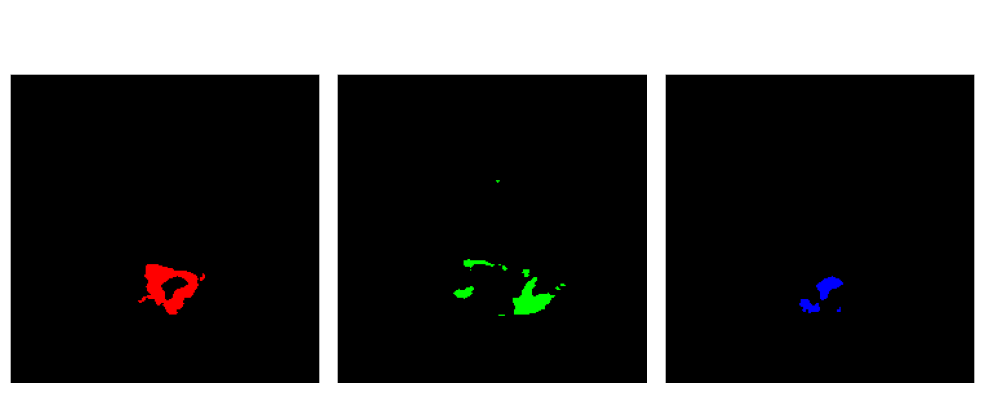
\includegraphics[width=0.85\textwidth]{segmentation-bin-prediction.png}}
			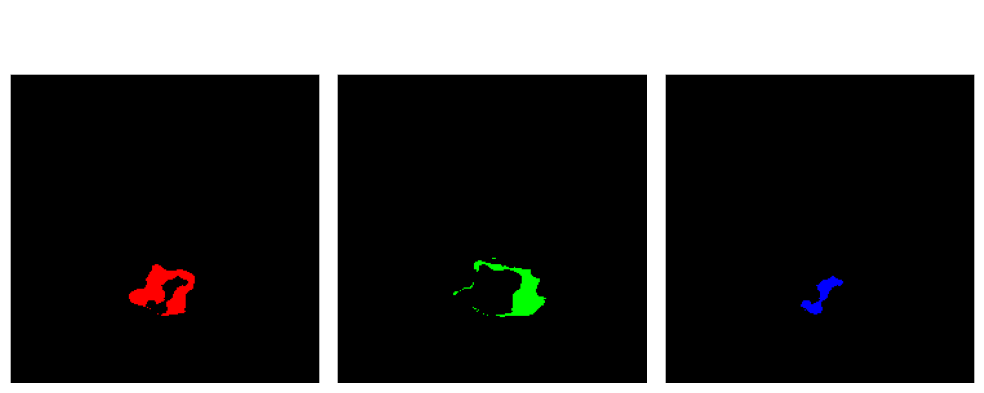
\includegraphics[width=0.85\textwidth]{segmentation-ground-truth.png}
		\end{figure}

\end{frame}


% Slide 7 ──────────────────────────────────────────────────────────────────────
\begin{frame}

	\frametitle{Performance Assessment}

	\begin{equation*}
		\begin{array}{c c c c c}
			\text{Dice} = \frac{2 \times |X \cap Y|}{|X| + |Y|} & 
			\quad\quad &
			\text{Precision} = \frac{TP}{TP + FP} & 
			\quad\quad &
			\text{Recall} = \frac{TP}{TP + FN} \\[1em]
			\substack{
				\text{\gray{\itt{Dice Coefficient}}} \\[0.5em]
				\text{\azure{\itt{``overlap'' metric}}}
			} & &
			\substack{
				\text{\gray{\itt{Precision}}} \\[0.5em]
				\text{\azure{\itt{prediction quality}}}
			} & &
			\substack{
				\text{\gray{\itt{Recall}}} \\[0.5em]
				\text{\azure{\itt{prediction quantity}}}
			}
		\end{array}
	\end{equation*}

	\vspace{2ex}

	\begin{figure}
		\centering
		\only<1>{
\includegraphics[width=\textwidth]{metrics-red.png}}%
		\only<2>{
\includegraphics[width=\textwidth]{metrics-green.png}}%
		\only<3>{
\includegraphics[width=\textwidth]{metrics-blue.png}}%
		\only<4>{
\includegraphics[width=\textwidth]{metrics-average.png}}
	\end{figure}

\end{frame}


% Slide 8 ──────────────────────────────────────────────────────────────────────
\begin{frame}

	\frametitle{Visualizing Attention Maps}
	
	\begin{figure}
		\centering
		
\includegraphics[width=\textwidth]{attention_maps.png}
	\end{figure}

\end{frame}

\end{document}

